% See http://www.ecn.purdue.edu/~mark/puthesis/#Options
% for documentclass options.
\documentclass[ece,dissertation]{puthesis}
\usepackage{amsmath}
\usepackage{multicol}
\usepackage{subfigure}

%\usepackage{graphicx}
%\usepackage{geometry}
%\usepackage{changepage}
\usepackage{tikz}
%\usepackage[titletoc]{appendix}
%\usepackage{titlesec}
%\usepackage{setspace}
%\usepackage{showframe}
%\usepackage{mathptmx}
%\usepackage{times}
%\usepackage{fancyhdr}
%\usepackage{url}

%\usepackage{algorithm}
\usepackage{algorithmic}

\usetikzlibrary{matrix,shapes,arrows,positioning,chains}

% Title of thesis (used on cover and in abstract).
\title{Outdoor Laser Guidance System Application\\
  for Precision Agriculture}

% First author name with first name first is used for cover.
% Second author name with last name first is used for abstract.
\author{Xiangnan Gong}{Gong, Xiangnan}

% First is long title of degree (used on cover).
% Second is abbreviation for degree (used in abstract).
% Third is the month the degree was (will be) awarded (used on cover
% and abstract).
% Last is the year the degree was (wlll be) awarded (used on cover
% and abstract).
\pudegree{Master of Science in Electrical and Computer Engineering}{MSECE}{May}{2017}

% Major professor (used in abstract).
% Use \majorprofs{...} if you have more than one professor.
\majorprof{Lingxi Li}

% Campus (used only on cover)
\campus{Indianapolis}

%
%  mydefs.tex  2007-03-19  Mark Senn  http://www.ecn.purdue.edu/~mark
%
%  Command definitions that can be used in all documents that have
%      %
%  mydefs.tex  2007-03-19  Mark Senn  http://www.ecn.purdue.edu/~mark
%
%  Command definitions that can be used in all documents that have
%      %
%  mydefs.tex  2007-03-19  Mark Senn  http://www.ecn.purdue.edu/~mark
%
%  Command definitions that can be used in all documents that have
%      \input{mydefs}
%

% CHANGE NEXT 3 LINES?
% Define \be and \ee to start and end the equation environment.
\newcommand{\be}{\begin{equation}}
\newcommand{\ee}{\end{equation}}

% CHANGE NEXT 12 LINES?
% Define \Repeat so, for example,
%     \Repeat{whatever}{10}
% is the same as typing whatever 10 times.
\newcount{\myi}
\newcommand{\Repeat}[2]{%
    \myi=0
    \loop
        \ifnum\myi<#2
        #1
        \advance\myi by 1
    \repeat
}

% CHANGE NEXT 3 LINES?
% Make "\Sum ab" or "\Sum{a}{b}" do "\sum_{a}^{b}".
% This can only be used when in math mode.
\newcommand\Sum[2]{\sum_{#1}^{#2}}

% CHANGE NEXT 4 LINES?
% Make "\xn" do "$x_n$".
% Because this definition contains the "$" to go into math mode
% this definition must be used when not in math mode.
\newcommand{\xn}{$x_n$}

% CHANGE NEXT 5 LINES?
% Since \xn is already defined we must use \renewcommand to redefine it.
% Normally you would not have the above definition for \xn in this file
% if you were just going to override it later.
% The \ensuremath goes into math mode if not already in math mode.
\renewcommand{\xn}{\ensuremath{x_n}}
%

% CHANGE NEXT 3 LINES?
% Define \be and \ee to start and end the equation environment.
\newcommand{\be}{\begin{equation}}
\newcommand{\ee}{\end{equation}}

% CHANGE NEXT 12 LINES?
% Define \Repeat so, for example,
%     \Repeat{whatever}{10}
% is the same as typing whatever 10 times.
\newcount{\myi}
\newcommand{\Repeat}[2]{%
    \myi=0
    \loop
        \ifnum\myi<#2
        #1
        \advance\myi by 1
    \repeat
}

% CHANGE NEXT 3 LINES?
% Make "\Sum ab" or "\Sum{a}{b}" do "\sum_{a}^{b}".
% This can only be used when in math mode.
\newcommand\Sum[2]{\sum_{#1}^{#2}}

% CHANGE NEXT 4 LINES?
% Make "\xn" do "$x_n$".
% Because this definition contains the "$" to go into math mode
% this definition must be used when not in math mode.
\newcommand{\xn}{$x_n$}

% CHANGE NEXT 5 LINES?
% Since \xn is already defined we must use \renewcommand to redefine it.
% Normally you would not have the above definition for \xn in this file
% if you were just going to override it later.
% The \ensuremath goes into math mode if not already in math mode.
\renewcommand{\xn}{\ensuremath{x_n}}
%

% CHANGE NEXT 3 LINES?
% Define \be and \ee to start and end the equation environment.
\newcommand{\be}{\begin{equation}}
\newcommand{\ee}{\end{equation}}

% CHANGE NEXT 12 LINES?
% Define \Repeat so, for example,
%     \Repeat{whatever}{10}
% is the same as typing whatever 10 times.
\newcount{\myi}
\newcommand{\Repeat}[2]{%
    \myi=0
    \loop
        \ifnum\myi<#2
        #1
        \advance\myi by 1
    \repeat
}

% CHANGE NEXT 3 LINES?
% Make "\Sum ab" or "\Sum{a}{b}" do "\sum_{a}^{b}".
% This can only be used when in math mode.
\newcommand\Sum[2]{\sum_{#1}^{#2}}

% CHANGE NEXT 4 LINES?
% Make "\xn" do "$x_n$".
% Because this definition contains the "$" to go into math mode
% this definition must be used when not in math mode.
\newcommand{\xn}{$x_n$}

% CHANGE NEXT 5 LINES?
% Since \xn is already defined we must use \renewcommand to redefine it.
% Normally you would not have the above definition for \xn in this file
% if you were just going to override it later.
% The \ensuremath goes into math mode if not already in math mode.
\renewcommand{\xn}{\ensuremath{x_n}}
\newcommand{\margins}{\Repeat{Show where the margins for the page are.}{4}}
\let\en=\ensuremath
\newcommand{\ve}[2]{\en{#1_1},~\en{#1_2},\ \ldots,~\en{#1_{#2}}}

\begin{document}

\volume

% Front matter (dedication, etc.).
%
%  revised  front.tex  2017-01-08  Mark Senn  http://engineering.purdue.edu/~mark
%  created  front.tex  2003-06-02  Mark Senn  http://engineering.purdue.edu/~mark
%
%  This is ``front matter'' for the thesis.
%
%  Regarding ``References'' below:
%      KEY    MEANING
%      PU     ``A Manual for the Preparation of Graduate Theses'',
%             The Graduate School, Purdue University, 1996.
%      PU8    ``A Manual for the Preparation of Graduate Theses'',
%             Eighth Revise Edition, Purdue University.
%      TCMOS  The Chicago Manual of Style, Edition 14.
%      WNNCD  Webster's Ninth New Collegiate Dictionary.
%
%  Lines marked with "%%" may need to be changed.
%

  % Statement of Thesis/Dissertation Approval Page
  % This page is REQUIRED.  The page should be numbered page ``ii''
  % and should NOT be listed in your TABLE OF CONTENTS.
  % References: PU8 ordinal pages 5 and 29.
  % The web page https://engineering.purdue.edu/AAE retrieved on
  % January 8, 2017 had "School of Aeronautics and Astronautics"---that
  % is used instead of "Department af Aeronautics and Astronautics"
  % below.
\begin{statement}
  \entry{Dr.~Lingxi Li, Chair}{Department of Electrical and Computer Engineering}
  \entry{Dr.~Brian King}{Department of Electrical and Computer Engineering}
  \entry{Dr.~Maher Rizkalla}{Department of Electrical and Computer Engineering}
  \approvedby{Dr.~Brian King}{Head of the Electrical and Computer Engineering Graduate Program}
\end{statement}

  % Dedication page is optional.
  % A name and often a message in tribute to a person or cause.
  % References: PU 15, WNNCD 332.
%\begin{dedication}
%  This is the dedication.
%\end{dedication}

  % Acknowledgements page is optional but most theses include
  % a brief statement of apreciation or recognition of special
  % assistance.
  % Reference: PU 16.
\begin{acknowledgments}
  I would like to thank my advisor for his guidance and encouragement through the research and writing process. I am grateful to all of my committee members for the time and energy they have put into helping me complete my research. 
	
	\bigskip
	My family and friends kept me motivated and happy during this long process.
	
	\bigskip
	Your support means so much to me. Thank you.
\end{acknowledgments}

  % The preface is optional.
  % References: PU 16, TCMOS 1.49, WNNCD 927.
%\begin{preface}
%  This is the preface.
%\end{preface}

  % The Table of Contents is required.
  % The Table of Contents will be automatically created for you
  % using information you supply in
  %     \chapter
  %     \section
  %     \subsection
  %     \subsubsection
  % commands.
  % Reference: PU 16.
\tableofcontents

  % If your thesis has tables, a list of tables is required.
  % The List of Tables will be automatically created for you using
  % information you supply in
  %     \begin{table} ... \end{table}
  % environments.
  % Reference: PU 16.
\listoftables

  % If your thesis has figures, a list of figures is required.
  % The List of Figures will be automatically created for you using
  % information you supply in
  %     \begin{figure} ... \end{figure}
  % environments.
  % Reference: PU 16.
\listoffigures

  % List of Symbols is optional.
  % Reference: PU 17.
\begin{symbols}
  $m$& mass\cr
  $v$& velocity\cr
\end{symbols}

  % List of Abbreviations is optional.
  % Reference: PU 17.
\begin{abbreviations}
  abbr& abbreviation\cr
  bcf& billion cubic feet\cr
  BMOC& big man on campus\cr
\end{abbreviations}

  % Nomenclature is optional.
  % Reference: PU 17.
%\begin{nomenclature}
%  Alanine& 2-Aminopropanoic acid\cr
%  Valine& 2-Amino-3-methylbutanoic acid\cr
%\end{nomenclature}

  % Glossary is optional
  % Reference: PU 17.
%\begin{glossary}
%  chick& female, usually young\cr
%  dude& male, usually young\cr
%\end{glossary}

  % Abstract is required.
  % Note that the information for the first paragraph of the output
  % doesn't need to be input here...it is put in automatically from
  % information you supplied earlier using \title, \author, \degree,
  % and \majorprof.
  % Reference: PU 17.
\begin{abstract}
  Currently, there are many types of Automatic Guided Vehicles (AGVs) in different industries. Typically their job is to move raw materials or parts around a manufacturing facility, and they can be very accurate by following the guides from wires in the floor, magnets, laser, or vision. However, currently AGVs only work indoors. Therefore, the purpose of this thesis is to discuss the implementation of the outdoor AGV. An outdoor AGV has much more constraints than an indoor one. The environment indoors can be easily controlled while the outdoor cannot because there could be such problems as rough outdoor surfaces, no pre-set guiding wires or magnets, vision blocking by dust, and so on. The solution, which will be introduced in this paper, to achieve the outdoor AGV is laser guidance. In addition, a buffer will be installed to stabilize the cargo or others working devices, to prevent them from the shaking due to the rough outdoor surfaces. To be more specific, a prototype will be built to simulate the working of a seeder. In agriculture, it is very important to plant corns in a straight line, not only to increase the absorption of sunlight and ventilation, but also to reduce the work of irrigation, fertilizing, and harvest. Furthermore, to achieve unmanned agriculture, a corn field with straight lines will also be a good condition for other agriculture robots.
\end{abstract}


%
%  revised  introduction.tex  2011-09-02  Mark Senn  http://engineering.purdue.edu/~mark
%  created  introduction.tex  2002-06-03  Mark Senn  http://engineering.purdue.edu/~mark
%
%  This is the introduction chapter for a simple, example thesis.
%


\chapter{Introduction}

Since the nineteenth century, machines have been playing more and more important roles in every aspect all around the world. Especially in modern factories, a few workers with a well-designed mechanical production line are capable to accomplish the job that used to require hundreds of skilled workers to do . Specifically, machines brought to us not just efficiency, but also accuracy and reliability. Therefore, automatizing production—or, rather, replacing human workers with robots—is imperative for every production plant.


\section{Introduction to Indoor AGVs and Their Guidance Systems}

In the 1950s, the first Automatic Guided Vehicle (AGV)—a tow truck following a wire in the floor—was introduced by Barrett Electronics to handle materials for a production line. \cite{olmi2011traffic} However, after decades of development, AGVs are able to help achieve the unmanned production line in many factories. Modern AGVs with built-in microprocessors can be controlled by computer. Therefore they are not only able to move heavy materials around, but they are also significantly accurate and reliable. A typical AGV can have over $1,000$ pounds of load capacity; in addition, the tracking accuracy is just $\pm 1.27 cm$. \cite{KESH} 
		
There are many types of AGVs, such as towing vehicles, unit load carriers, forklift trucks, and so on. They all move around factories by following guidance systems.  
		
%\section{Current AGVs}
The most popular guidance systems for current indoor AGVs are wire-guided, optical, inertial, infrared, laser, and teaching type. \cite{KESH}

\begin{itemize}
    \item Wire-Guided:
    \begin{itemize}
    \item An energized wire is rooted along the guide path. 
    \item The antenna of the AGV follows the rooted wire.
    \end{itemize}
    %The outdoor crop field is very large compared to the indoor factories. It is too expensive to root wire under ground in advance. And because of the variety of the temperature and humidity, the wire is easy to be eroded.
    \item Optical:
    \begin{itemize}
    \item Colorless florescent particles are painted on the concrete/tiled floor. 
    \item Photosensors are used to track these particles.
    \end{itemize}
    %It is impossible to paint the colorless florescent particles on the soil.
    \item Inertial:
    \begin{itemize}
    \item The guide path is programmed on a microprocessor that is fixed on the AGV. 
    \item A sonar system is incorporated for finding obstacles.
    \end{itemize}
    %Sonar system cannot be used as a guide system in an open area.
    \item Infrared:
    \begin{itemize}
    \item Infrared light transmitters are used to detect the position of the vehicle.
    \item Reflectors are affixed on the top of the vehicle to reflect the light.
    \end{itemize}
    %It is hard to detect the position of the vehicle by using infrared light transmitters in under sunlight.
    \item Laser:
    \begin{itemize}
    \item A laser beam is used to scan wall-mounted bar-coded reflectors.
    \item Accurate positioning can be obtained.
    \end{itemize}
    %This is using for a very close distance to enhance accuracy.
    \item Teaching type:
    \begin{itemize}
    \item The AGV learns the guide path by moving along the required route.
    \item The AGV sends the information to the host computer.
    \end{itemize}
    %The outdoor ground is rough and unpredictable. It is hard to stay in the planned route by just memorizing it. Because small errors of moving on rough ground cumulates to big errors. 
\end{itemize}
%It is obvious that none of the indoor AGVs guide systems are suitable for outdoor AGVs.

In general, the guide could be pre-rooted wire, magnet, or colorless florescent particles of paint. All of these AGVs are fairly accurate, but they can only work indoors. Wires and magnets need to be planted underground, and paint needs to be painted on concrete or tiled floor. The indoor environment can be well controlled, while an outdoor environment cannot because it is very complicated and unpredictable. The ground could be rugged, wet, or steep, and because the terrain is exposed, it is susceptible to cold or rain, as well as dust, light, and the Earth's magnetic field. This paper will provide a solution to bring AGVs from indoor to outdoor use, and introduce AGV to the field of precision agriculture.

\section{Introduction to Outdoor Farm Machinery and Their Guidance Systems}

%引入介绍农业机械的导航系统
For thousands of years, farming has been one of the most important methods to harvest food. There has been a big leap from traditional farming, where the farmer could only get help from cattle or horses, to modern farming, where the farmer could get help from farm machinery. It is possible to satisfy the explosive food demand of the world's human population because of the development of farming technology.

Combine harvesters are one of the most famous farm machinery. They are well-known for their efficiency and convenience. The traditional procedure of harvesting wheat is cutting, sheaving, drying, threshing, and winnowing. On a modern farm, the whole process can be done by a combine harvester, which is a big leap forward for harvesting crops. However, modern farming is not only about harvesting; it is also about tilling, seeding, watering, fertilizing, and so on. And all the rest of this work is done by tractors and appropriate attachments.
\begin{figure}[ht!]
\begin{center}
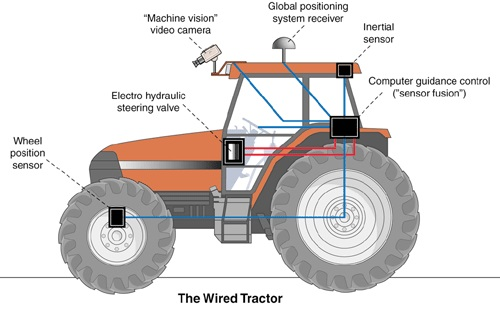
\includegraphics[scale = 1]{pics/GPStractor.jpg}
\caption{Tractor With GPS Guidance System}
\end{center}
\end{figure}

Tractor is the core machine of field work. It can do different jobs with different attachments. Figure  1.1 shows a modern tractor with many sensors installed. The most significant one is the GPS receiver. The GPS guidance system is one of the most popular guidance systems that works outdoors. Under the help of a GPS guidance system, the field usage efficiency can be optimized. However, the accuracy of GPS is always a problem. Although there is a improved solution for GPS, which has brought the accuracy to centimeter level, the cost becomes very expensive.

\section{Importance of Subject}

Labor is one of the most significant factors of agriculture. With the help of farm machinery, the total amount of labor dedicated to farming has decreased by about 30 percent for hired labor and about 40 percent for self-employed labor from 1982 to 2007. Moreover, the farm output increased by 35 percent (Table 1.1) while the total amount of labor dedicated to farming was decreased. \cite{o2011changing} %So the machines are really good helpers to farm. 
\begin{table}[ht!]
\begin{center}
\caption{The Change Labor and Output in Agriculture}
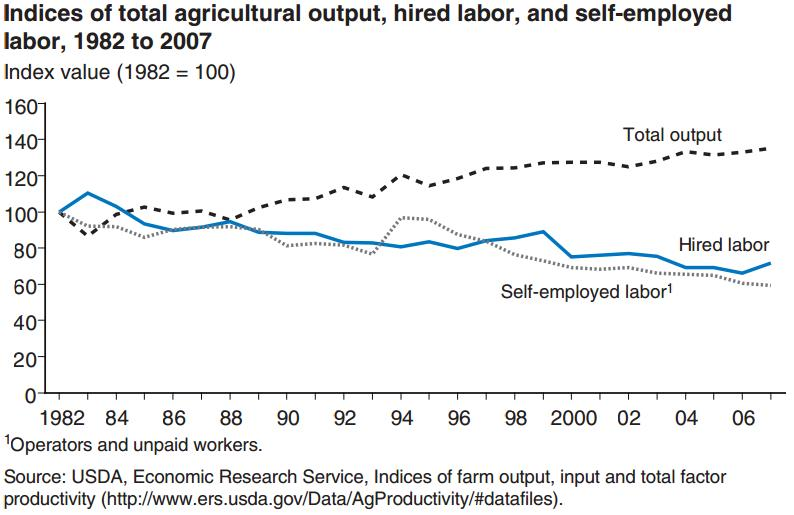
\includegraphics[scale = 0.7]{pics/laborandoutput.jpg}
\end{center}
\end{table}
Undoubtedly, the usage of farm machinery not only lowers the amount of labor, but also increases the productivity. 

In late 20th century, Pierre Robert proposed, developed, and popularized precision agriculture. \cite{mcbratney2005future} Most of the farm machinery now has the GPS, which stands for Global Positioning System, on board because of his contribution. It is very easy to plant all crops in nicely columns with the GPS guidance system. GPS-mounted farm machinery did a great job in the past few years, but there is a problem. The accuracy of the original GPS is typically about a few meters. Fortunately, a technology improved the accuracy to $\pm$ 10 $cm$. \cite{thuilot2002automatic} Although this $\pm$ 10 $cm$ accuracy is acceptable with most popular 76.2 $cm$ row spacing, not for 50.8 $cm$ or 38.1 $cm$ row spacings that will be used in the future. \cite{fawcett2014farm} And the experiment field has an even higher requirement. The objective of the experiment field is to find the highest quality breed of crops. Therefore, it is extremely important to keep the growth environment of every plant at the same level, and the position to seed the experiment field is strict. Every plant should be kept at the same distance to one other, which is the precondition to provide every plant the same amount of water, sunlight, fertilizer, and carbon dioxide. Failure to do this will cause the result of the experiment to be meaningless. As a result, it is vital to have outdoor AGVs working as accurately as the indoor ones.

\section{Knowledge Gap}

Currently in the United States, the products of modern farming not only fulfill food demand of the United States, but also surpass it. For example, more than 70 percent of the volume of U.S. production of Cotton and Tree nuts were exported from 2011 to 2013 (Table 1.2). And the overall average annual export share of U.S. agricultural production is 20 percent since 2000. \cite{Exports}
\begin{table}[ht!]
\begin{center}
\caption{Export Share of U.S. Farm Production, 2011-13}
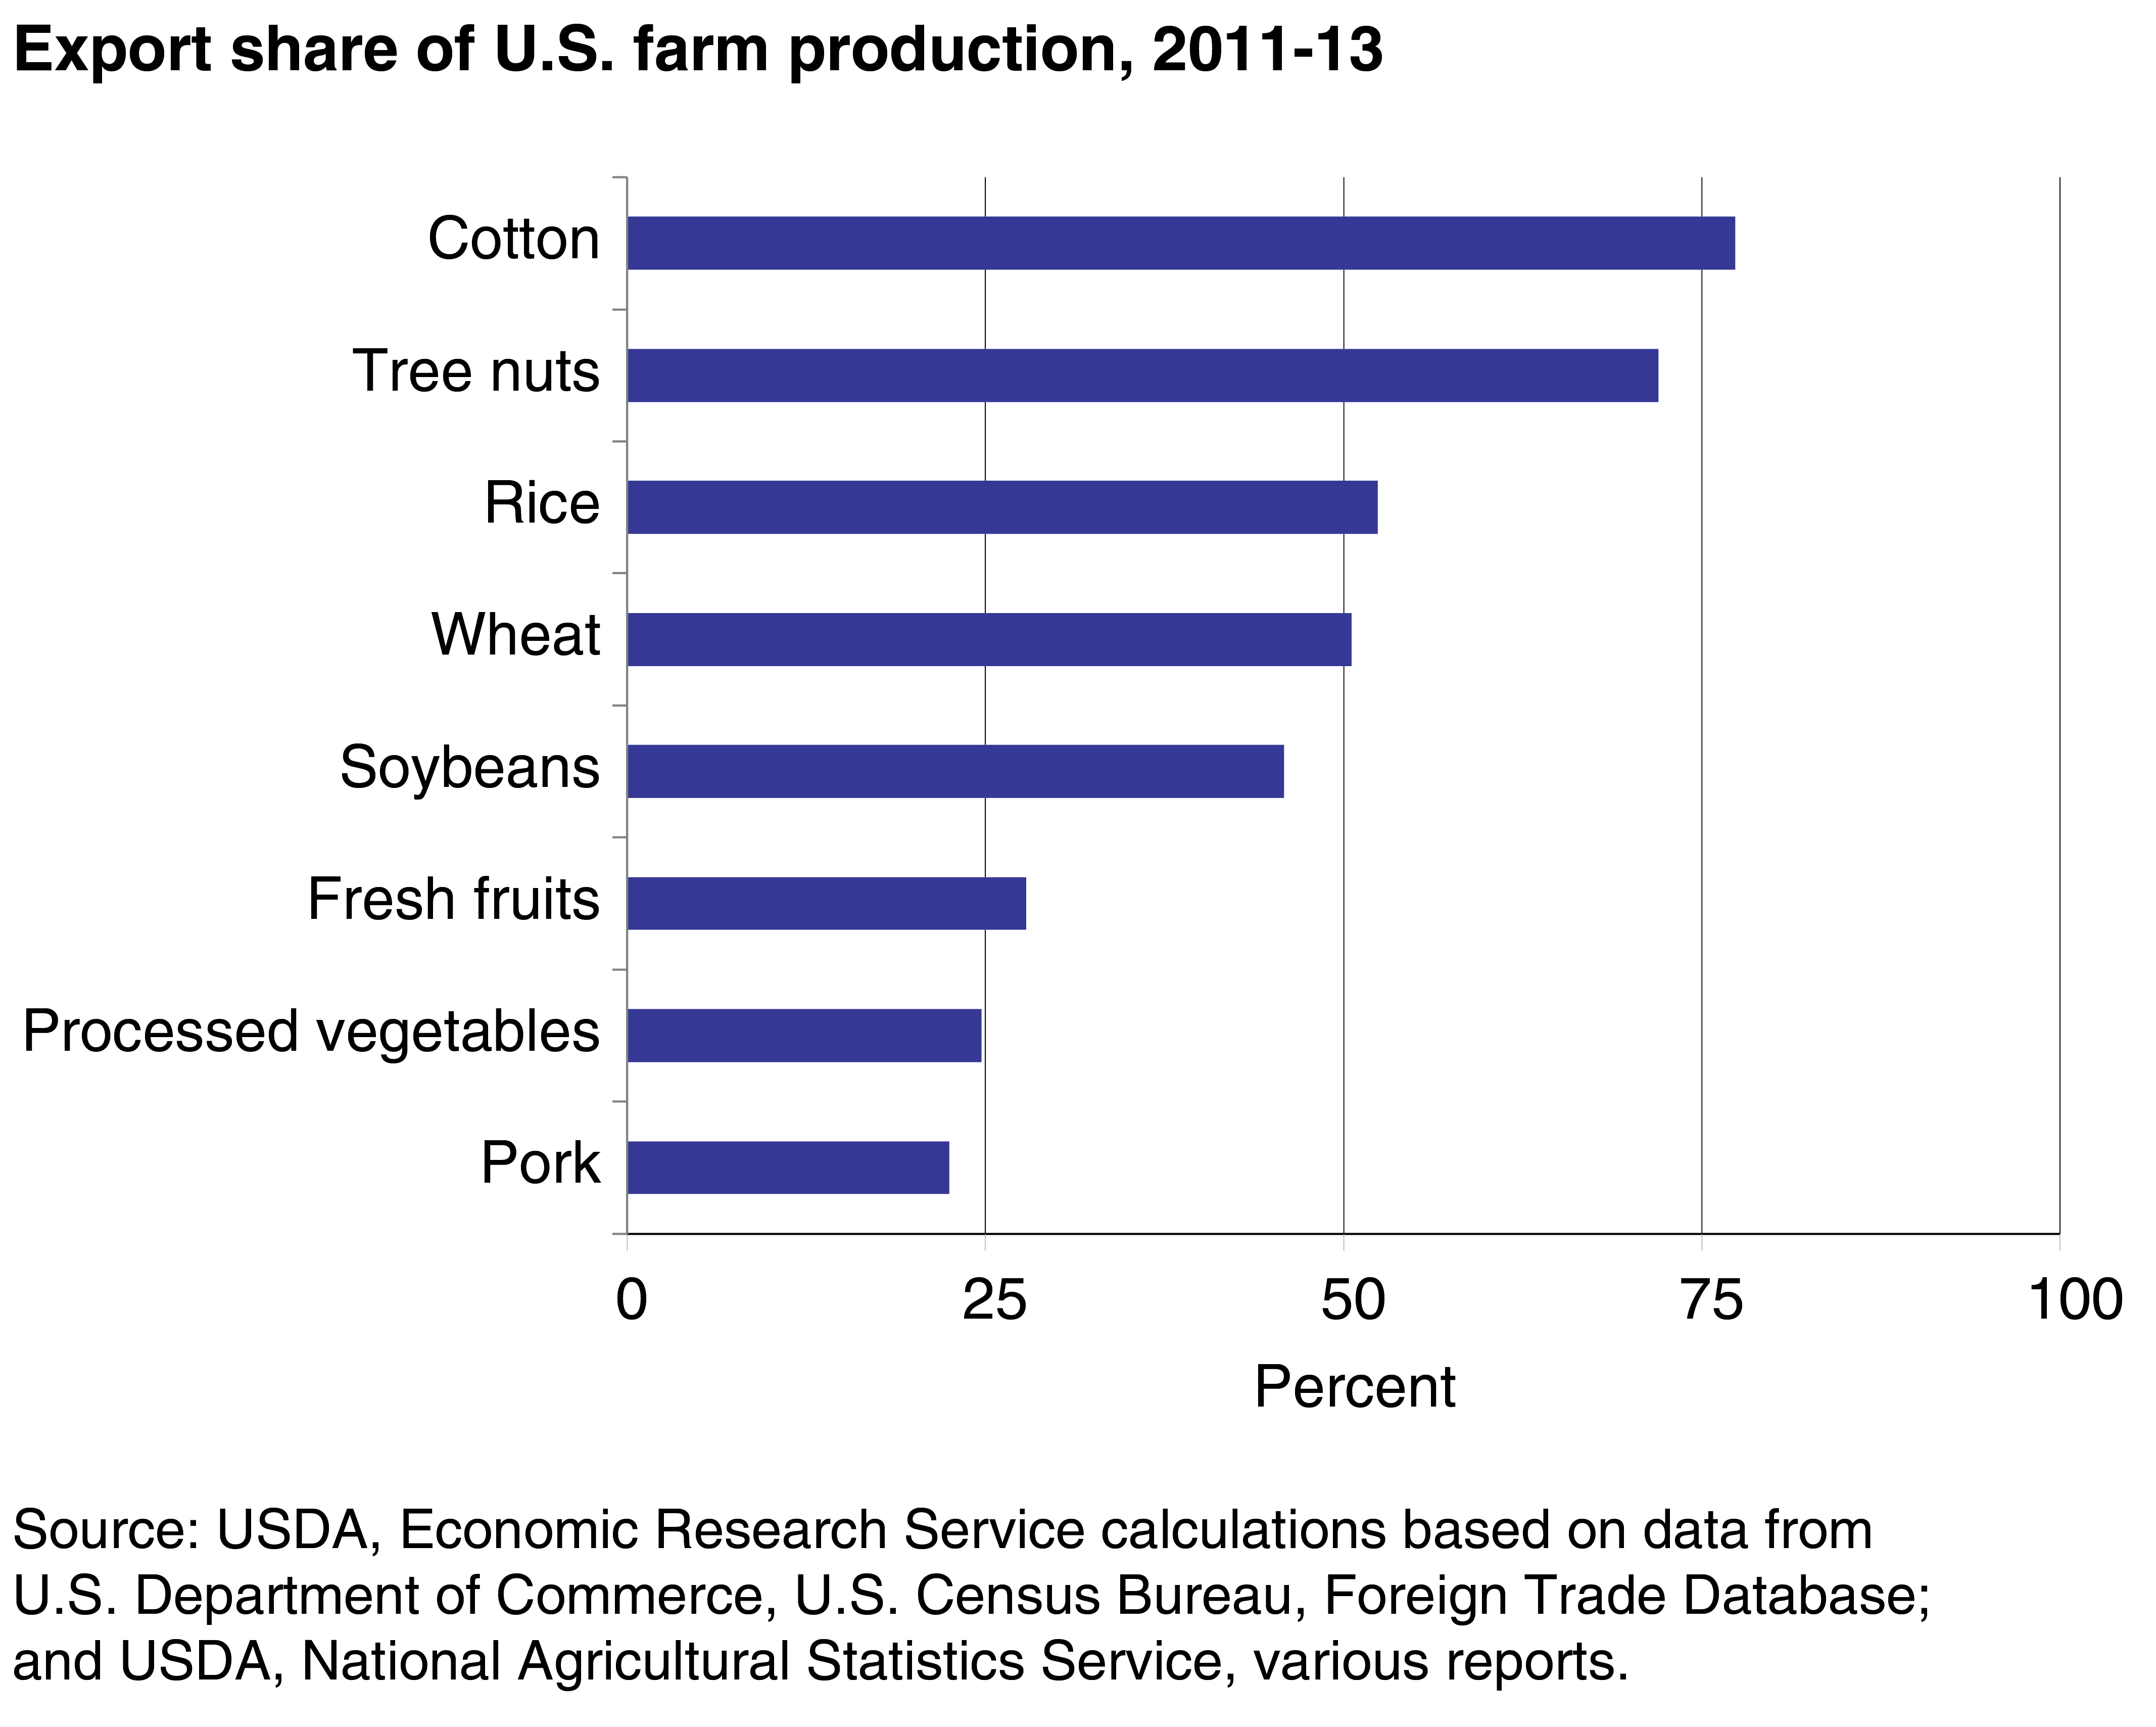
\includegraphics[scale = 0.4]{pics/cropexport.png}
\end{center}
\end{table}
Since there is no food shortage in the United States, the technology of farm machinery seems to be more than enough. However, there are many other places in the world where it is very hard to grow crops, because the farming conditions are totally different compared to North America. 
\subsection{Situations Which Require Higher Accuracy}
The water scarcity in West Asia and North Africa is a well-known problem. The world average annual per capita renewable supplies of water was about $7000 m^{3}$ in 1999; however, it was below $1500 m^{3}$ in West Asia and North Africa at the same time. More seriously, this level was $3500 m^{3}$ in 1960, and it was expected to continuously decrease to less $700 m^{3}$ by the year of 2025. \cite{margat1999water} One of the best solutions for water scarcity is to use micro-irrigation, or more specifically, drip irrigation (Figure 1.2). 
\begin{figure}[ht!]
\begin{center}
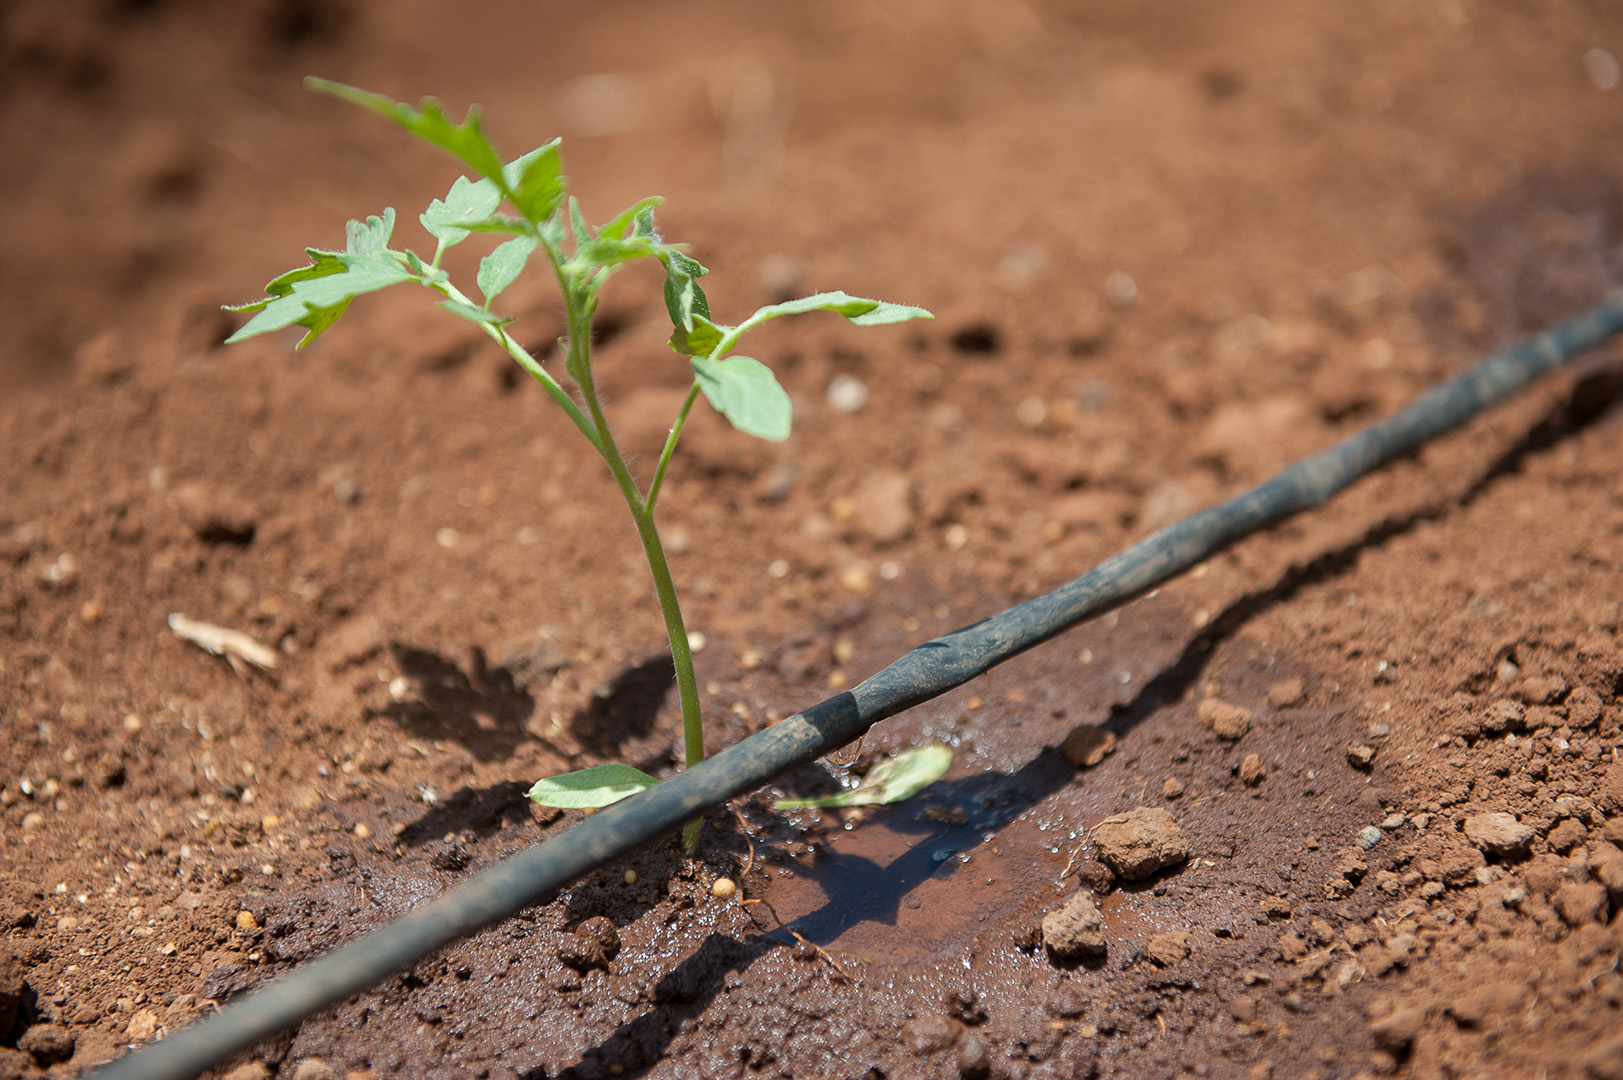
\includegraphics[scale = 0.2]{pics/drip.jpg}
\caption{Drip Irrigation}
\end{center}
\end{figure}
Some advantages of micro-irrigation include improved water and nutrient management, potential for improved yields and crop quality, greater control of applied water resulting in less water and nutrient loss through deep percolation, and reduced total water requirements. \cite{phene1986advantages} Unfortunately, the applications of micro-irrigation is also limited. Mostly, micro-irrigation is used on permanent plantings such as trees and vines. The reason that it is not used on the field crops is that it needs to be installed and removed at the beginning and the end of each growing season. Furthermore, field corps are different from trees and vines; their height is low, so the working zone is close to the ground. Therefore, the drip tubes make the other fields operations more difficult than it used to be. An improved method to make it possible to use micro-irrigation on field corps is to bury the tubes underground. \cite{camp1998subsurface} Although the tubes neither affect the field operations nor need to be reinstalled every growing season, the position of the drip spot is fixed once it is buried. So the problem turns into planting crops in the right position, which can be solved by the outdoor AGV that this paper introduces. 

\subsection{Situations Which Require Lower Cost}

The development of China is not comprehensive, and farming especially is not developed. Table 1.3 show the difference of cereals productivity between China and the United States. The cereals productivity of China is only 75.4\% compare to the United States. However, the labor dedicated for agriculture is about 300 million in China, while this number is only about 2 million in the United States. The disparity in this number shows that the per capita arable land is only about $0.3 hm^{2}$ in China, while it is about $61 hm^{2}$ in the United States. \cite{tao2012}
\begin{table}[ht!]
\begin{center}
\caption{Cereals Productivity}
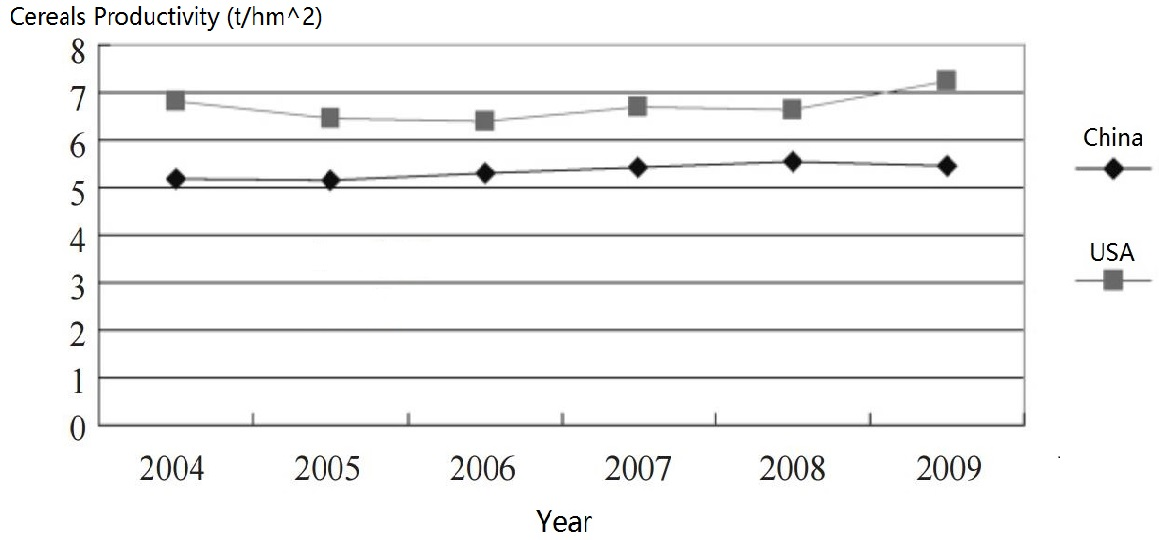
\includegraphics[scale = 0.4]{pics/tperhm.jpg}
\end{center}
\end{table}
\begin{table}[ht!]
\begin{center}
\caption{Labor Dedicated For Agriculture}
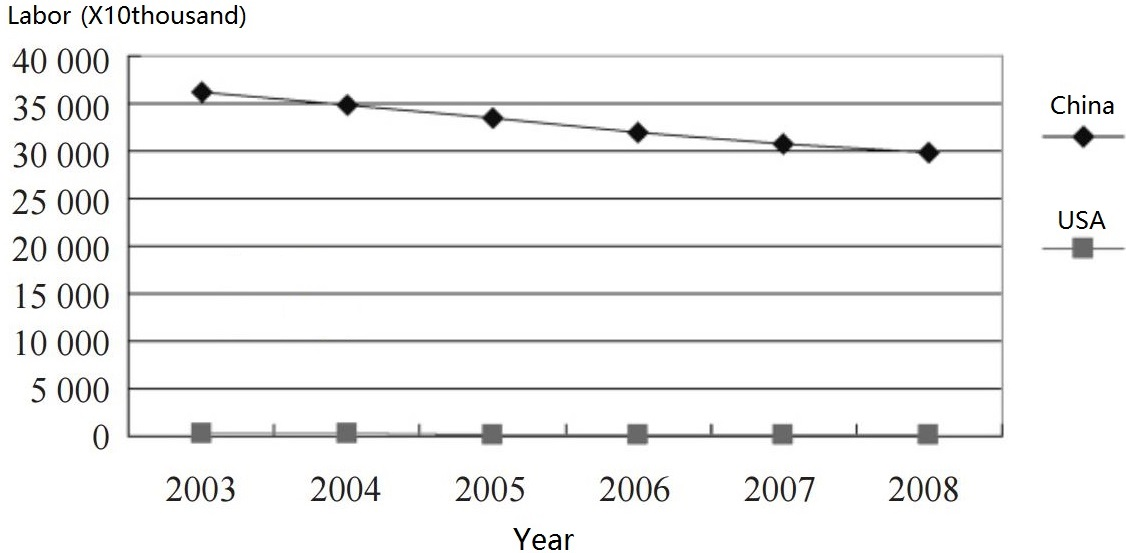
\includegraphics[scale = 0.4]{pics/10k.jpg}
\end{center}
\end{table}
\begin{table}[ht!]
\begin{center}
\caption{Per Capita Arable Land}
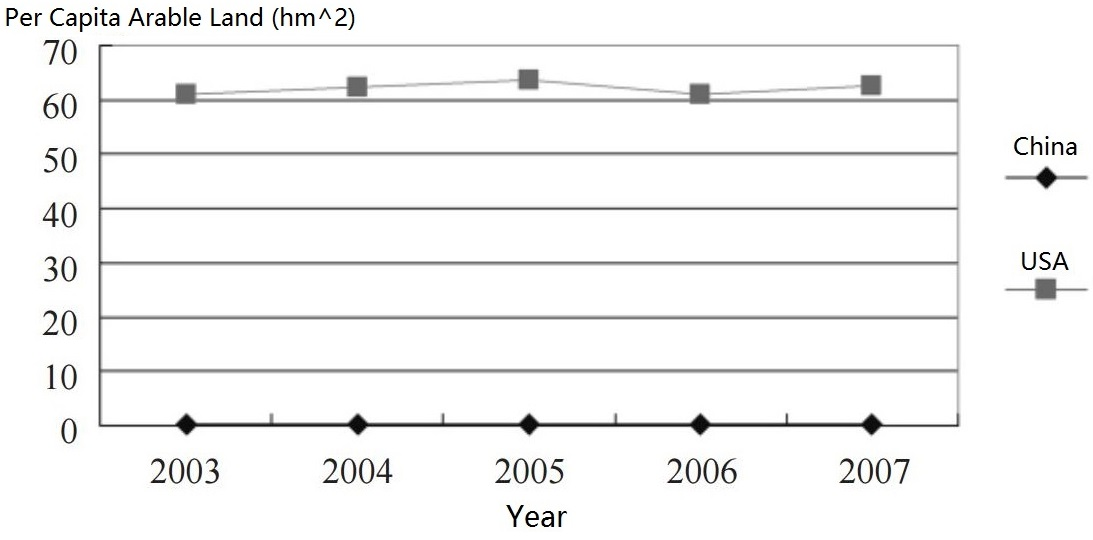
\includegraphics[scale = 0.4]{pics/capitahm2.jpg}
\end{center}
\end{table}
The inefficient productivity and scarcity of arable land brought poverty to Chinese farms. The average net income per capita of Chinese rural family is as low as 7916.6RMB in 2012, which is about 1250USD. \cite{income2012} 

Agriculture in China is dramatically different than in the United States. Although the agricultural structure in China has been modernizing for years, it is still rare to see  modern farm machinery in the field. This situation is caused by two reasons. First, the arable land for each farmer is too small to use big machines, and it is small enough so that the traditional ways still work. The second reason is that the annual income for each rural family is too low to buy a big machine. A basic agriculture tractor with 50-75 horsepower is typically from \$20,000 to \$40,000.\cite{tractorcost} And the GPS units cost vary from different systems. Basic WAAS light bars cost about \$2,000 with accuracy from 12 to 15 inches. The RTK GPS units typically cost \$12,000 to \$25,000, plus a \$750 to \$1,500 annual subscription service fee.\cite{PriceR} This is much more than what a Chinese rural family can afford. 





\chapter{RELATED RESEARCH}

\section{GPS}
GPS guidance systems are one of the most reliable guidance systems. There are many advantages to GPS, such as low cost, portability, and able to work anywhere without any pre-installation. However, the accuracy of GPS has always been a problem for agriculture. An experiment in 2014 found a result: 
\begin{quote}
almost half (49.6\%) of all ≈68,000 GPS points recorded with the Qstarz Q1000XT GPS units fell within 2.5 m of the expected location, 78.7\% fell within 10 $m$ and the median error was 2.9 $m$. The four different types of areas showed considerable variation in the median error: 0.7 $m$ in open areas, 2.6 $m$ in half-open areas and 5.2 $m$ in urban canyons. \cite{schipperijn2014dynamic}
\end{quote}
According to this research, the median error for GPS is 0.7 $m$ in open areas, which is 70 $cm$. This accuracy is obviously not enough for field operations because row spacing is 76.2 $cm$.

\section{Improved GPS guidance}
An improved technology for GPS, CP-DGPS (Carrier Phase Differential GPS) or RTK GPS (Real-Time Kinematic GPS), brought the accuracy to centimeter level. This RTK GPS has two receivers; one is called \textit{reference}, while another is called \textit{rover}. \textit{Reference} is a receiver that is installed to a fixed position, which is the base station in Figure 2.1. It always stays at the same position and permanently receives satellite signals, calculates its ‘GPS’ position and determines the difference with the coordinates attributed to its own position. The \textit{rover} is mobile and placed where it is needed. It receives both GPS signals from satellites and the correction values from the \textit{reference} via radio signals. The accuracy of RTK GPS is around 2-3 $cm$. \cite{lambiel2004contribution} However, the ground condition of crop fields is unpredictable, so the 2-3 $cm$ accuracy for GPS does not equate to 10 $cm$ accuracy for tractors. It is infeasible for the large tractor to do centimeter-level adjustment.
\begin{figure}[ht!]
\begin{center}
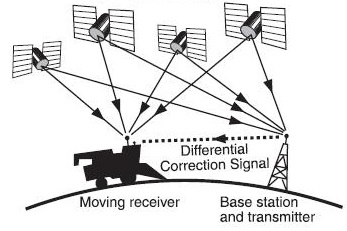
\includegraphics[scale = 1.1]{pics/RTGPS.jpg}
\caption{Real-Time Differential GPS}
\end{center}
\end{figure}
In fact, the error is about 10 $cm$ based on an experiment with a large farm tractor. \cite{thuilot2002automatic} 
%This error is acceptable with most popular 76.2 $cm$ row spacing now, but not for the 50.8 $cm$ or 38.1 $cm$ row spacing in the future. \cite{fawcett2014farm} 

\section{Vision-Based Guidance}

Vision-based guidance is an efficient way to improve the actual accuracy and lower the cost of using precision GPS. There are two methods; 3D imaging and color detection. They are both limited. The 3D imaging method detects the height of crops, so it cannot work on young crops. The color detection method finds the color of crops. However, the color of crops may vary from crop to crop and season to season. A recent study introduced a new method called image processing. The new algorithm uses the parallel texture of crop rows as the reference. \cite{english2014vision} (Figure 2.2)

\begin{figure}[ht!]
\begin{center}
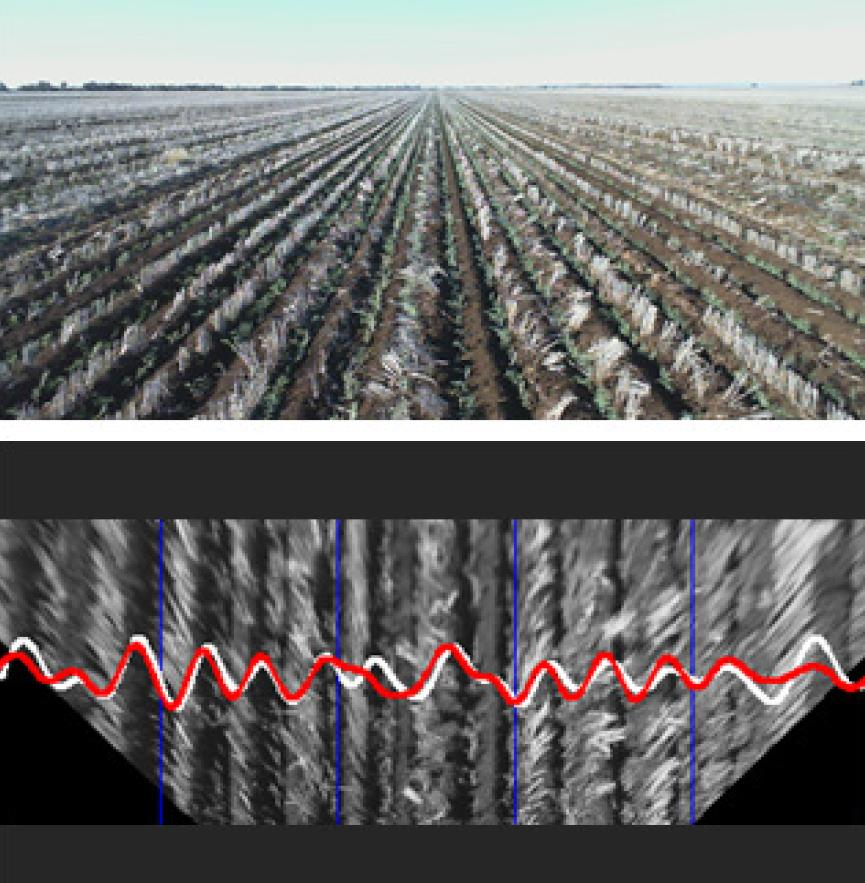
\includegraphics[scale = 0.45]{pics/parallel.jpg}
\caption{Parallel Texture}
\end{center}
\end{figure}

The result shows the accuracy is mostly lower than 10 $cm$. Therefore, this low-cost, vision-based guidance may be a very competitive alternative solution to precision GPS in the future. However, there is one fatal flaw: 
\begin{quote}
The largest diversion at around 300m occurs while the robot is driving at an angle over a contour bank (raised ridge for diverting water). The rows are likely to not have been straight in this location since GPS guided tractors commonly do not compensate for the tilt of the vehicle as they drive at an angle over contour banks causing the planted rows to wobble.

The wheat and chickpeas datasets shows the least offset error which we attribute to the narrow spacing and relatively clear crop template. \cite{english2014vision}
\end{quote}

Therefore, it needs nice parallel rows to work. It is difficult for a tractor, even with precision GPS, to create these parallel rows because GPS-guided tractors do not compensate for sliding and tilt.

\section{Sliding Correction}
Unlike asphalt roads, soil cannot provide constant friction on each tire of a vehicle. Sliding is a significant problem that causes trajectory errors. Therefore an algorithm for sliding estimation was developed. Two inclinometers were installed on the vehicle to collect data. (Figure 2.2) 
\begin{figure}[ht!]
\begin{center}
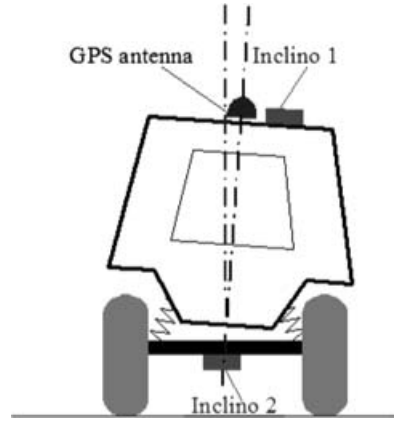
\includegraphics[scale = 0.4]{pics/slidingcorrection.png}
\caption{Position of Inclinometers}
\end{center}
\end{figure}
From these two tilt angles, the design algorithm can estimate the sliding and then give feedback to the control system for correction. The result from this research is shown in Table 2.1. \cite{lenain2006high}
\begin{table}[ht!]
\caption{Deviation Signal Properties}
\begin{center}	
\begin{tabular}{|l|l|l|}
\hline
 & Without sliding incorporated & Without sliding incorporated \\ 
\hline
Mean & 4 cm & -3 cm \\
\hline
Std &  30 cm & 8 cm\\
\hline
In $\pm$15 cm & 29\% & 90\%\\
\hline

\end{tabular}
\end{center}					
\end{table}

\chapter{RESEARCH PROBLEMS}


Although some cites in China, such as Beijing and Shanghai, are well-known magnificent modern cities and the GDP of China was ranked number two in the world in 2015 \cite{GDP2015}, agriculture is a short plate of China's modernization. According to the current situation in China, Chinese farmers are unable to afford neither big farm machinery, nor precision GPS guidance systems. Since the arable land and annual income is only about 0.3$hm^{2}$ and 7916.6RMB for each farmer, small and cheap farm machinery is the best choice. A common farm tractor in the United States is normally 50-75 horsepower, while the popular ones in China are only about 20 horsepower. The price for a small tractor with 20 horsepower is about 13,000RMB (about 1950USD), which is affordable for one family or several together. However, the cost for an agricultural GPS guidance systems is too much; farmers in China cannot afford them. The WAAS GPS offers the lowest cost, but 2,000USD is enough for another small tractor. (Table 3.1) 
\begin{table}[ht!]
\caption{GPS Guidance Systems and Prices \cite{PriceR}}
\begin{center}	
\begin{tabular}{|l|l|l|}
\hline
NAME & ACCURACY & Estimated Price \\ 
\hline
WAAS & 12 to 15 inches & \$2,000 \\
\hline
WAAS with AutoSteer &  12 to 15 inches & \$4,000\\
\hline
OmniStar & sub-meter & \$6,000 + \$1,150 per year\\
\hline
Radio Beacon & - & \$12,500\\
\hline
RTK & 1 inch & \$18,500 + \$1,125 per year\\
\hline
\end{tabular}
\end{center}					
\end{table}

In addition, WAAS only works in the United States. These differences between the China and the United States mean that it is infeasible to develop agriculture in China the same way that it is in the United States. Therefore, finding an accurate and low-cost alternative solution for planting crops in parallel rows is the first step to achieve the modern farming and precision agriculture in China.

Based on the related researches and the situations in China, achieving precision agriculture means not only improving the accuracy of the trajectory of farm machinery, but also lowering the cost of guidance systems. Therefore, the research problem of this paper is to find a low-cost solution that improves the accuracy of a tractor's trajectory. The idea of reducing cost is to implement an add-on device that is compatible to any of the existing farm tractors, so that farmers can just pay a small amount of money to upgrade their own tractor. 

%Based on the related researches, achieving precision agriculture is not only to improve the accuracy of the position of farm machinery, but also to improve the accuracy of the trajectory of tractor. With the localization technology, correction could be made once the vehicle off the track; with the sliding estimation technology, correction could be made once the tire slid. All the researches have done were trying to find the exact position of the tractor or to estimate sliding of it then make the correction. However, making correction means errors already occurred. To prevent error from happening, an additional device and guide system was designed.

\chapter{LASER GUIDANCE SYSTEM DESIGN}

\section{Laser Guidance System Overview}
Driving on the farm field faces unpredictable ground conditions all the time, such as rocks, mounds, slides, or rabbit or rat holes. It is impossible for tractors to drive through every thing without deviating from the planned track. However, it is possible to have the attachments of the tractors always stay on the planned track. In order to do so, a physical buffer is designed to be installed on the tractor attachment, and the frame of all the tools on the attachment should connect to the buffer so that they move along with the buffer. Therefore, this buffer is able to keep the field tools independent from the tractor and always on the planned trajectory.
\begin{figure}[ht!]
\begin{center}
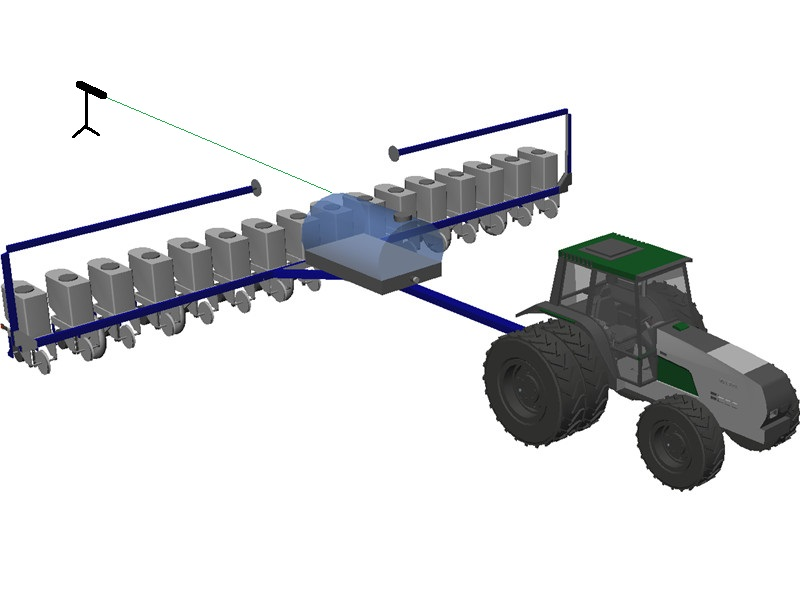
\includegraphics[scale = 0.6]{pics/tractor.jpg}
\caption{Laser guide}
\end{center}
\end{figure}

According to the related researches, vision guidance has been chosen to use as the guidance system for the buffer, because a camera is a low-cost device. In this paper, an additional laser pointer is used as a stable reference. The laser pointer is placed at the end of rows facing to the back of the tractor to provide the guidance (Figure 4.1), so that the buffer can provide a proper compensation to deviation by observing the laser beam. 

In addition, two LEDs can be installed on both the left and right side of the dashboard of the tractor. The LEDs tell the driver to turn the steering wheel left or right to counter the deviation. 
%It is expected to improve the accuracy dramatically from 10 $cm$ to about 2 $cm$. 

%流程图
%增加论点:在驾驶室加装指示灯,这样可使没有任何导航系统的拖拉机精确移动

\section{Physical Buffer}

%描述buffer程序设计
\begin{figure}[ht!]
\begin{center}
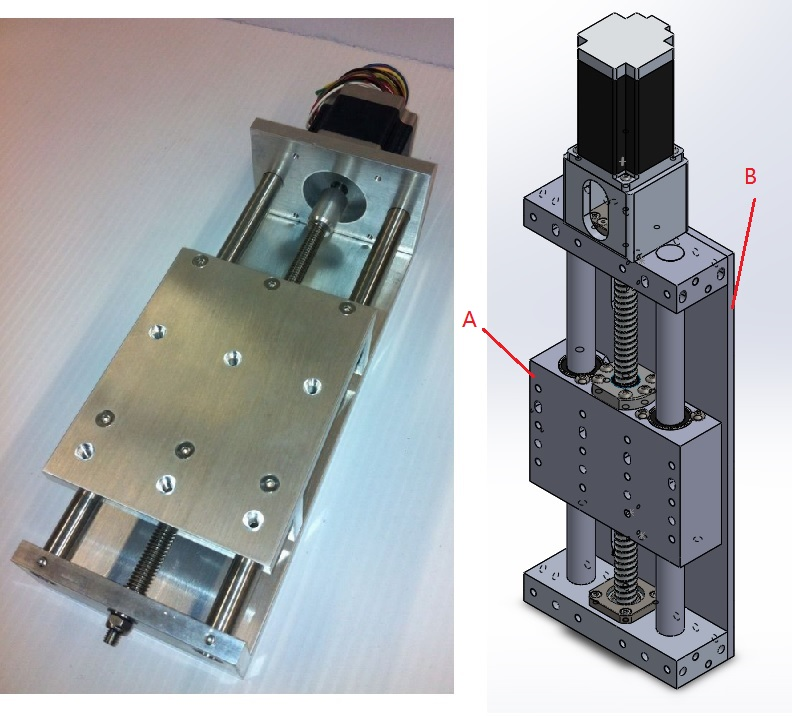
\includegraphics[scale = 0.6]{pics/1D.jpg}
\caption{Linear Sliding Track}
\end{center}
\end{figure}
The design for the physical buffer is to use the linear sliding track (Figure 4.2). There are two sides of the linear sliding track, as the CAD shows in Figure 4.2. Side A connects to the tractor and side B connects to the camera and attachment tools. In addition, considering tractor attachments very heavy, the sliding track must be firm and the stepper motor must be powerful. The physical buffer is installed on the tractor attachments. (Figure 4.3)
\begin{figure}[ht!]
\begin{center}
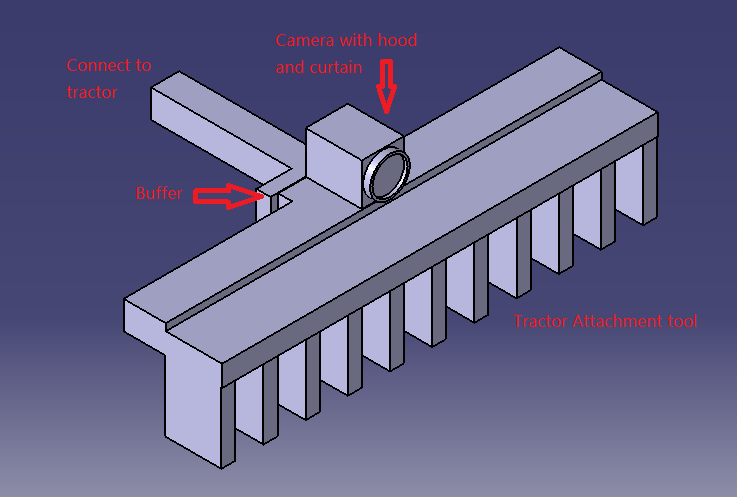
\includegraphics[scale = 0.8]{pics/attachmentwithbuffer.png}
\caption{Tractor with Buffer Installed}
\end{center}
\end{figure} 

The buffer allows the tractor to have some left or right displacement by providing an offset in the opposite direction to the attachment. Therefore, as long as the tractor moves in the right direction and has an accuracy within the offset range of the buffer, the attachment is able to work in a relatively stationary condition. 

\section{Image Processing}
\begin{figure}[ht!]
\begin{center}
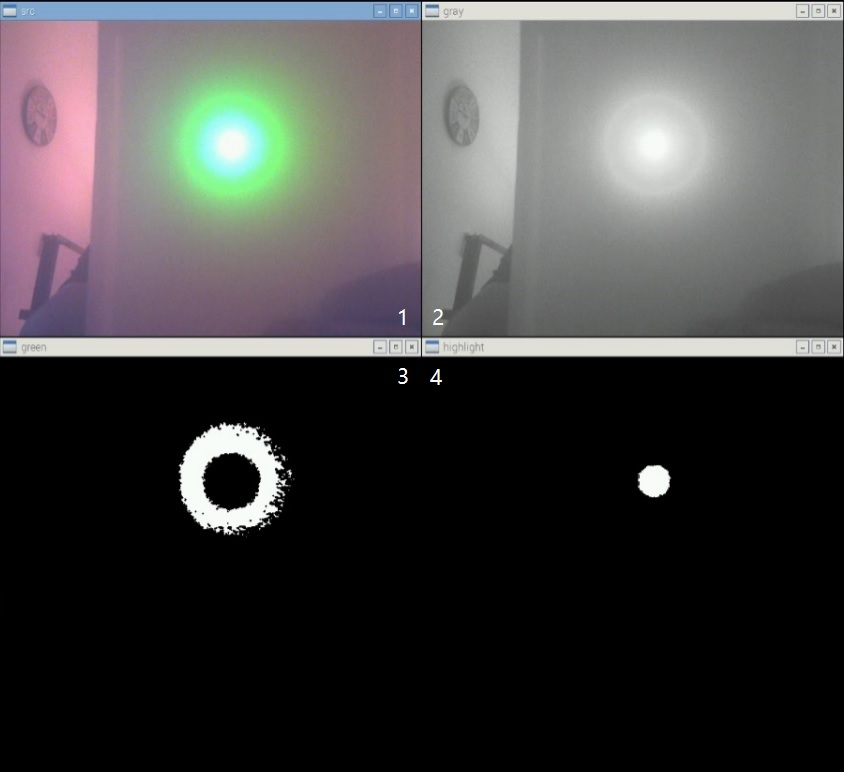
\includegraphics[scale = 0.7]{pics/imaging.jpg}
\caption{Image Processing}
\end{center}
\end{figure}
An image processing algorithm is using to find the position reference from the data gathered by the camera. The algorithm was written in C++ with OpenCV. Several different options were tested.

\subsection{Color Detection}

Color detection was the first method that was implemented and tested. Color detection is straightforward and accurate. Generally, green should be a great color for detection because green has the lowest showing frequency in our daily life, which is why chroma key compositing technology always uses green as the background color. However, green could be everywhere in a crop field, so it is hard to detect the green laser with a green background. To solve this problem, a hood and curtain were attached to the camera to reduce the low intensity lights. Therefore, only the green laser was able to leave a clear green spot on the sight of the camera. (Figure 4.4 - 1) Although the spot is clear green from human vision, it may not be recognized as green by camera. Under the RGB color space, the "green" spot is always mixed with blue, and sometime red. The color detection is very unreliable, because it could be affected by the surrounding light, thickness of the curtain, and other unknown factors.
\subsection{Improved Color Detection}

According to a related research, the HSV color space has achieved a more accurate performance compared to the original RGB color space. \cite{kaur2013content} To improve the color detection, HSV color space was tested. RGB is well known as red, green, and blue, which are the primary colors of light. Every pixel on a picture contains these three values. Similar to RGB, the three values of HSV are hue, saturation, and value. Unlike the RGB color space where every value has a range from 0 to 255, the values of the HSV color space have different ranges. Hue is the color type, which ranges from 0 to 360 degree. Both saturation and brightness, which is value, range from 0 to 100 percent. The RGB color space is based on the Cartesian coordinate system, but the HSV color space is based on the cylindrical coordinate system. (Figure 4.5)
\begin{figure}[ht!]
\begin{center}
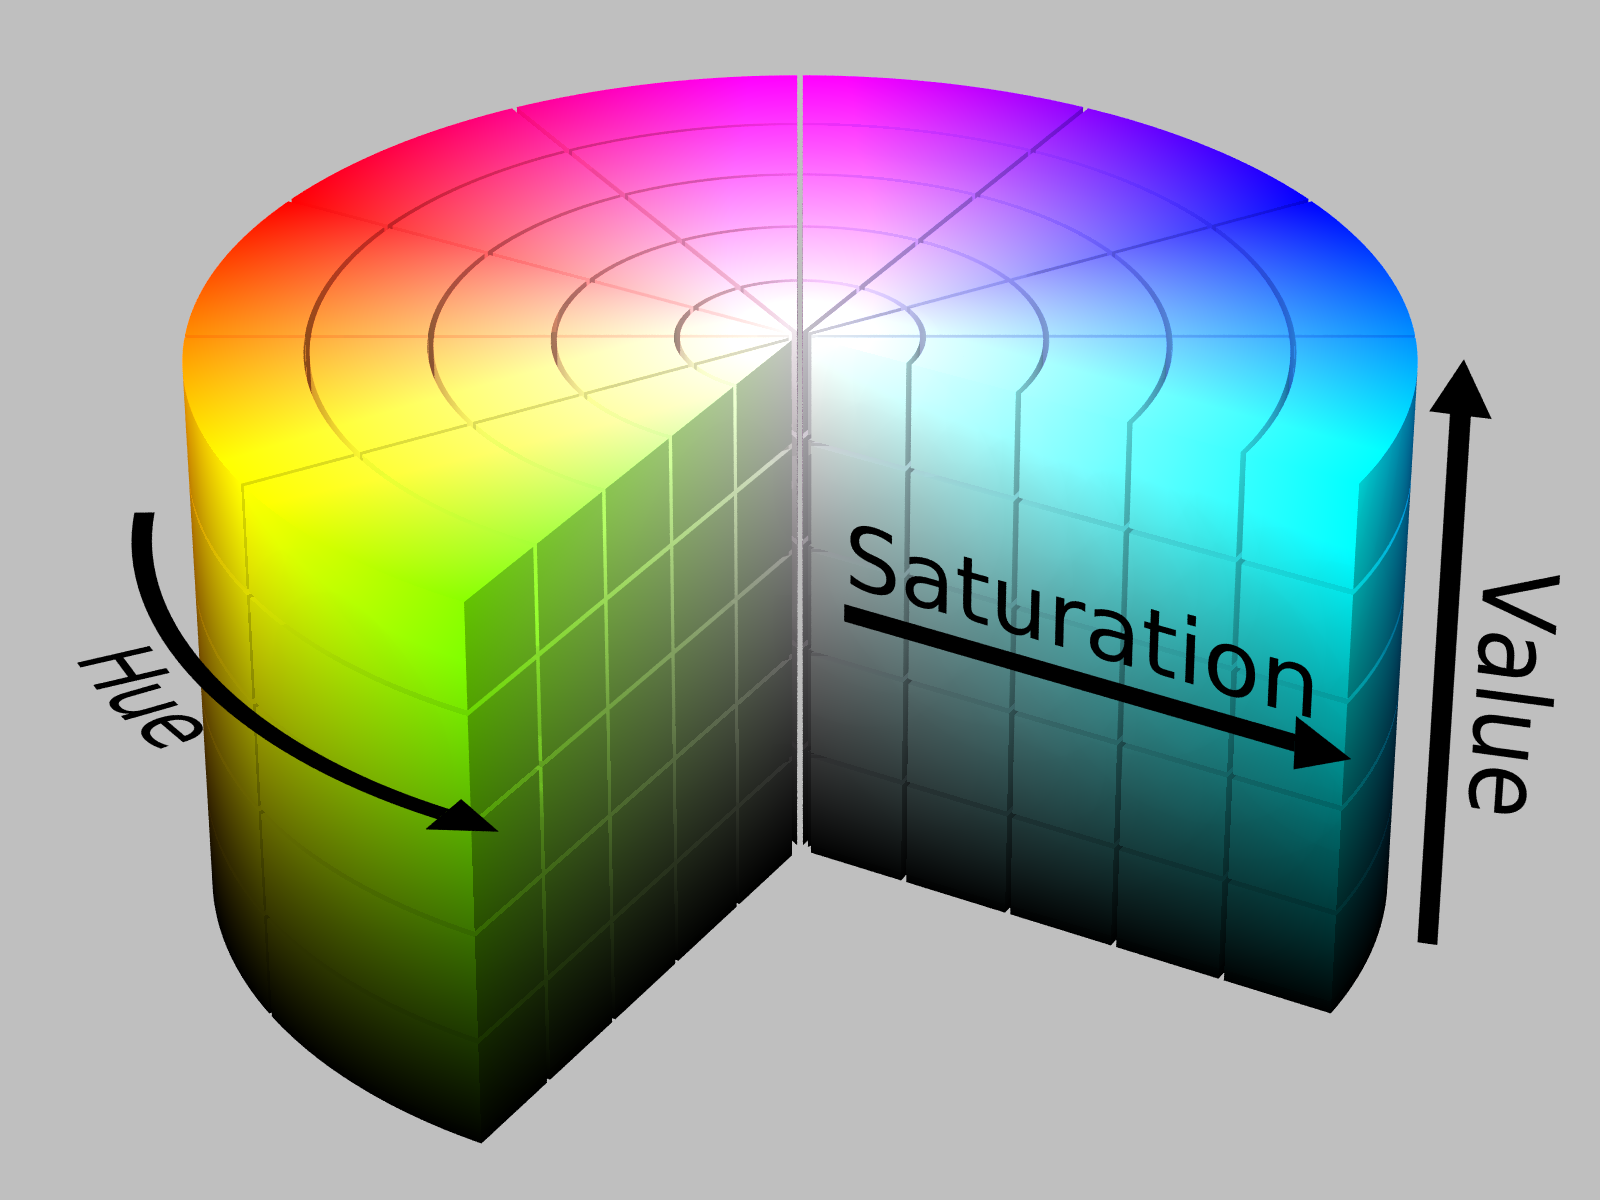
\includegraphics[scale = 0.2]{pics/HSV.png}
\caption{HSV Color Space}
\end{center}
\end{figure}

The conversion formulas are,
\begin{equation}
H = cos^{-1}(\frac{\frac{1}{2}[(R-G)+(R-B)]}{\sqrt{(R-G)^{2}+(R-B)(G-B)}})
\end{equation}
\begin{equation}
S = 1-\frac{3}{R+G+B}(min(R,G,B))
\end{equation}
\begin{equation}
V = \frac{1}{3}(R+G+B)
\end{equation}
After the original image transferred from RGB to HSV, a ring-shaped detection was showing on the screen. (Figure 4.4 - 3) The green color detection was stable in the HSV color space, but the ring-shaped detection was unable to provide an accurate coordinate. Unfortunately, there is no way to detect green at the center, because the light intensity at the center is too high for the camera to detect any color.
\subsection{High-Intensity Detection}

For close-distance detection, an additional algorithm was developed. This algorithm only  provides an accurate detection in a close range in order to help color detection. First, the original image was transferred from RGB to GRAY instead of HSV. (Figure 4.4 - 2) Then find the intensity bump was found by masking off all the pixels that were 20 units lower than the maximum intensity. As a result, the detection became a nice point. (Figure 4.4 - 4)

\section{Control Law Design}
This algorithm is defined in the flow chart in Figure 4.6. At the beginning, the camera on the buffer sees the laser spot and sets up the initial position. As the tractor moves, the camera will keep detecting the current position and comparing it with the initial position. Once the left deviation is detected, the buffer will provide the right offset, and the LED on the right will be turned on to tell the driver to turn slightly right. Once the right deviation is detected, the buffer will provide the left offset, and the LED on the left will be turned on to tell the driver to turn slightly left.  In other words, this add-on device will maintain the laser spot in the original position and will notify the driver about detected deviations. 
% Define block styles
\tikzstyle{decision} = [diamond, draw, text width=2.5cm, text badly centered]
\tikzstyle{block} = [rectangle, draw, text width=3cm, text centered, rounded corners, minimum height=1cm]
\tikzstyle{line} = [draw, -latex']
\begin{figure}[ht!]
\begin{center}
\begin{tikzpicture}
\node[block](start) {Start};
\node[block, below = 1 of start] (origin) {Initialize Position};
\node[coordinate, below = 1cm of origin] (cycle) {};
\node[block, left = 2 of cycle](off) {Turn LEDs off};
\node[decision, below = 2 of origin] (L) {Is left deviation detected?};
\node[block, left = 2 of L] (goR) {Provide right offset and turn right LED on};
\node[decision, below = 1 of L] (R) {Is right slide detected?};
\node[block, left = 2 of R] (goL) {Provide deviation offset and turn left LED on};
\node[coordinate, left = 1cm of goR] (left) {};
\node[coordinate, below = 1cm of R] (bottom) {};

\path [line] (start) -- (origin);
\path [line] (origin) -- (L);
\path [line] (L) -- node [anchor = south] {yes} (goR);
\path [line] (goR) -- (left) |- (off);
\path [line] (L) -- node [anchor = east] {no} (R);
\path [line] (R) -- node [anchor = south] {yes} (goL);
\path [line] (goL) -| (left) |- (off);
\path [line] (R) --  node [near start, anchor = east] {no} (bottom) -| (left) |- (off);
\path [line] (off) -- (cycle);
\end{tikzpicture}
\caption{Flow Chart}
\end{center}
\end{figure}

\chapter{PROTOTYPE DESIGN}


\section{Materials and Instruments}
This buffer is designed to be an implement base on current tractor attachments. In this paper, a prototype was developed for designing and experimental purposes, see Figure 5.1. 
\begin{figure}[ht!]
\begin{center}
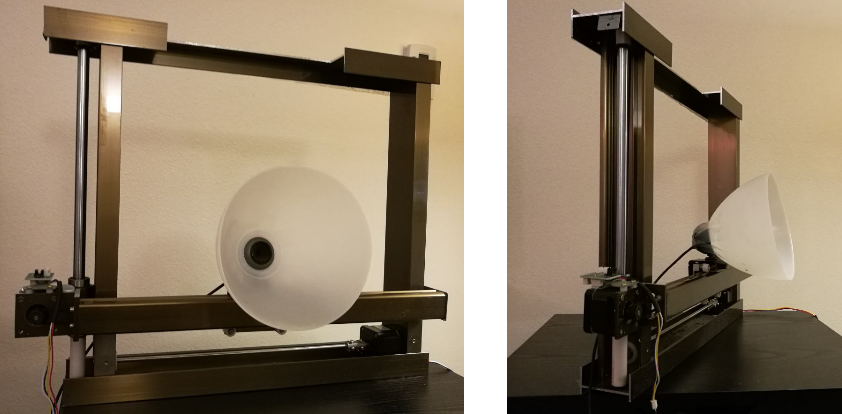
\includegraphics[scale = 0.6]{pics/prototype.png}
\caption{Prototype}
\end{center}
\end{figure}
A camera is installed on the top facing backwards to gather image information. A laser pointer is placed at the end of the row, facing the same direction as the tractor,  and aims at the camera while the tractor moves. Stepper motors are installed on the attachment's frame to offset the attachments, and a Raspberry Pi is used as the central processor to analyze the information gathered by the camera and to give the action commands to the stepper motors. In addition, stepper motor drivers boards are installed to transform the digital control signal to the stepper motors' input. The power supply was designed to use the battery of the tractor, so there is no battery in this prototype. All the parts are listed in Table 5.1.

\begin{table}[ht!]
\begin{center}	
\caption{Parts List}
\begin{tabular}{|l|p{1.5cm}|p{4cm}|l|l|l|}
\hline
Part Name & Vendor & Description  & Unit Cost & Qty. & Sub Total \\ \hline
Camera & Logitech & 480P WEBCAM & - & - & -\\ 
\hline
Stepper Motor & ECOSS INC & Came with frame & - & - &\\ 
\hline
Driver boards & DROK & L298N Motor Drive Controller Board & 6.99 & 1 & 6.99\\
\hline
Microprocessor & CanaKit & Raspberry Pi 2 with Starter Kit & 84.99 & 1 & 84.99\\
\hline
Frames & ECOSS INC & X-Y Stage Table Bed &  169.00 & 1 & 169.00\\
\hline
Wires & Phantom YoYo & 40p Male to Female 40p Female to Female & 4.40 & 1 & 4.40\\
\hline
Camera Hood & - & Lampshade & - & - & -\\
\hline
Curtain & - & Foam Board & - & - & -\\
\hline
Laser Pointer & Fowll & 532 nm Green Laser & 22.99 & 1 & 22.99\\
\hline
Power Supply & Goodwill & Used Charger & 1.99 & 2 & 3.98\\
\hline
Total Cost & & & & & 292.35\\
\hline
\end{tabular}
\end{center}
\end{table}

%对现有农机进行改装,所以成本低。现在实验阶段使用的是,电源,树莓派,摄像头,步进马达,框架,幕布,激光。(做图表,列出成本)

\section{Hardware}

\subsection{Laser Pointer}

A laser pointer is an economic and efficient way to provide a straight and stable reference. Thus, laser guidance is selected to be the guidance system. In order to observe a clear laser reference far in the distance, a high-power laser is the best choice. On the other hand, there are safety problems with laser pointers. High-power laser pointers could damage the retina if they are too close. Based on this safety problem, the laser's power should be restricted. To achieve both low power and far range, a green laser was chosen because, since green light has a shorter wave length than red light, it is able to spread farther than red light with the same power. According to Table 5.2, the maximum eye hazard distance of a 5 $mW$ green laser pointer is only 16 $m$, and the maximum distance from the spot on the screen is over 300 $m$, which is far enough for a row in a crop field. Also the laser pointer can be simply powered by a 3 $V$ lithium battery, which is convenient and inexpensive. According to the above consideration and analysis, a 5 $mW$ green laser was selected.
\begin{table}[ht!]
\begin{center}
\caption{Laser Range}
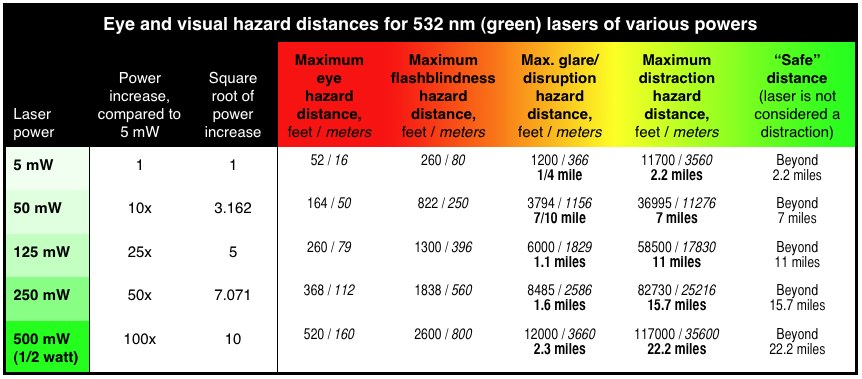
\includegraphics[scale = 0.5]{pics/laserrange.jpg}
\end{center}
\end{table}

\subsection{Buffer Design}


In this built prototype, a lighter and smaller frame was used for convenience. And for the demonstration purpose, no other heavy agricultural attachments will be installed. The camera was mounted on the small sliding block of the frame. Then, a hood was attached on the camera with a curtain covered in front. The hood reduces noise by blocking out light from the angle that the camera does not need to see. The curtain works like a projection screen, so that the laser pointer can leave a spot on it.  A stepper motor is installed on edge of the frame to drive the camera with a belt. The power of the stepper motor along with the control signal was given by a stepper motor driver board. 

The center processor is a Raspberry Pi, which processes the image captured by the camera and then sends the digital control signal to the stepper motor driver board. The wire connections are shown in Figure 5.2.
\begin{figure}[ht!]
\begin{center}
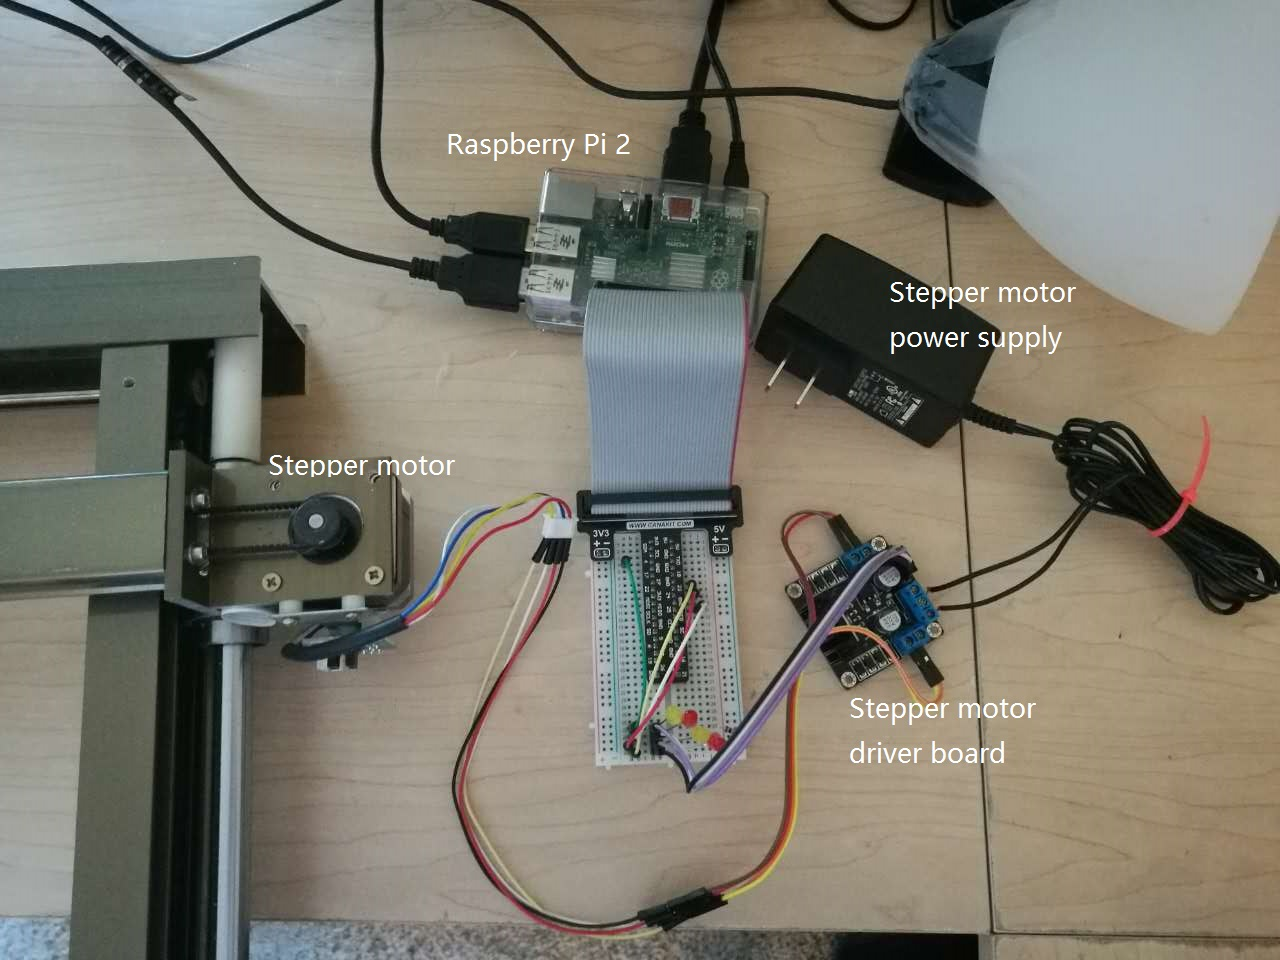
\includegraphics[scale = 0.4]{pics/connection.jpg}
\caption{Wire Connections}
\end{center}
\end{figure}
The prototype works based on the process shown in Figure 4.6. At the beginning, the laser pointer is pointed at the camera curtain. After the origin position is initialized, the frame is moved. The block with the camera, which may have other tractor attachment tools installed, will stay stable.

\section{Software}

\subsection{Image Processing on Raspberry Pi}
The image processing code on the Raspberry Pi was written by following the algorithm of section 4.3.2, with the green color detection based on the HSV color space, and 4.3.3, with the highest light intensity detection. 

Algorithm 1 shows the pseudo-code of green color detection. It blurs the source first to reduce the noise. The next source was converted from RGB color space to HSV color space. Then all the pixels out of the range were masked off, so there is only green color from the source left, which is turned to white. Then the masked image was eroded to minimize the white area. The last step was to find the centroid of the image.

Algorithm 2 works similarly, with two differences. First, the source was converted to GRAY instead of HSV. Second, the pixels other than the pixels that have the highest values were masked off all. 

The highlight detection algorithm dominates at first, and the green color detection algorithm will take over once it generates a steady result.

%\begin{algorithm}
%\caption{Green Color Detection}
\begin{algorithmic} 
\STATE {\textbf{Algorithm 1: Green Color Detection}}
\STATE {$blur(source)$}
\STATE {$green = BGR \rightarrow HSV(source)$}
\FOR {Every pixel of green}
\IF {$60 \leq H \leq 90, 90 \leq S \leq 255, 100 \leq V \leq 255$}
\STATE {$pixel = 255$}
\ELSE 
\STATE {$pixel = 0$}
\ENDIF
\ENDFOR
\STATE {$erode(green)$}
\STATE {$green point = centroid(green)$}				
\end{algorithmic}
%\end{algorithm}

%begin{algorithm}
%\caption{Highlight Detection}
\begin{algorithmic} 
\STATE {\textbf{Algorithm 2: Highlight Detection}}
\STATE {$blur(source)$}
\STATE {$gray = BGR \rightarrow GRAY(source)$}
\STATE {$max$ = max value of all pixel$(gray)$}
\FOR {Every pixel of gray}
\IF {$max-20 \leq pixel \leq max$}
\STATE {$pixel = 255$}
\ELSE 
\STATE {$pixel = 0$}
\ENDIF
\ENDFOR	
\STATE {$erode(gray)$}
\STATE {$highlight point = centroid(gray)$}			
\end{algorithmic}
%\end{algorithm}

\subsection{Stepper Motor Control on Raspberry Pi}

%		\begin{table}[ht!]
%			\begin{center}
%				\caption{Raspberry Pi Pins Layout}
%				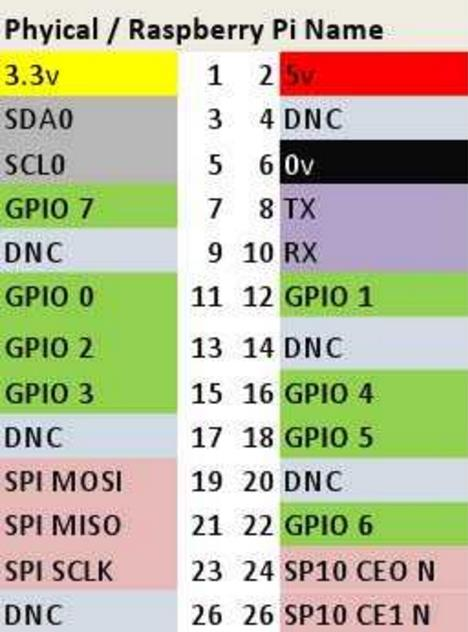
\includegraphics[scale = 0.5]{pipins.jpg}
%			\end{center}
%		\end{table}

%Table 5.3 shows the pins layout of Raspberry Pi. 
$GPIO 0,1,2,3$ is used as the digital signal output. Algorithm 3 is the pseudo-code for motor control. There is a user-defined function called rotate, which enables pin $0,1,2,3$ and initiates the signal sequence at the beginning. Next stepper motor is rotated for one revolution in the clockwise or counterclockwise direction depending on the input. The moving direction is determined by the main function, rotating clockwise if the $x$ coordinate of the point is less than or equal to 310 pixel, rotating counterclockwise if the if the $x$ coordinate of the point is greater than or equal to 330 pixel. And it do not move if the $x$ coordinate of the point is between 310 and 330 pixel. 

%\begin{algorithm}
%\caption{Motor Control}
\begin{algorithmic} 
\STATE {\textbf{Algorithm 3: Motor Control}}
\IF {$point.x \leq 310$}
\STATE {$rotate(clockwise)$}
\ELSIF {$point.x \geq 330$}
\STATE {$rotate(counterclockwise)$}
\ELSE
\STATE {do nothing}
\ENDIF 
%\STATE
\STATE {Function $rotate$($direction$)}
\STATE {$pins = 0, 1, 2, 3$}
\STATE {$sequence[8] = $}
%1, 1, 0, 0 \Rightarrow 0, 1, 0, 0 \Rightarrow 0, 1, 1, 0 \Rightarrow 0, 0, 1, 0 \Rightarrow 0, 0, 1, 1 \Rightarrow 0, 0, 0, 1 \Rightarrow 1, 0, 0, 1 \Rightarrow  1, 0, 0, 0$}
\STATE {$1, 1, 0, 0$}
\STATE {$0, 1, 0, 0$}
\STATE {$0, 1, 1, 0$}
\STATE {$0, 0, 1, 0$}
\STATE {$0, 0, 1, 1$}
\STATE {$0, 0, 0, 1$}
\STATE {$1, 0, 0, 1$}
\STATE {$1, 0, 0, 0$} 
\IF {$direction = clockwise$}
\FOR {$i = 1 \rightarrow 8$}
\STATE {$pins = sequence[i]$}
\ENDFOR
\ENDIF
\IF {$direction = counterclockwise$}
\FOR {$i = 8 \rightarrow 1$}
\STATE {$pins = sequence[i]$}
\ENDFOR
\ENDIF
\end{algorithmic}
%\end{algorithm}

\subsection{Multi-thread Programming}
%\begin{algorithm}
%\caption{Single Thread}
\begin{algorithmic} 
\STATE {\textbf{Algorithm 4: Single Thread}}
\LOOP
\STATE {Run image processing for one frame}
\IF {$point.x \leq 310$}
\STATE {$direction = clockwise$}
\ELSIF {$point.x \geq 320$}
\STATE {$direction = counterclockwise$}
\ELSE
\STATE {$direction =$ No move}
\ENDIF
\STATE {$rotate(direction)$}
\ENDLOOP		
\end{algorithmic}
%\end{algorithm}

Algorithm 4 was the original build for the software part of the laser guidance system; image processing and motor control is in the same loop. It is very inefficient because the clock frequency of the Raspberry Pi CPU is only 900MHz. Since the stepper motor can only rotate one revolution for each loop and the running time for image processing is much greater than motor control, the buffer hardly moves. It may have to rotate for hundreds of revolutions for each result to move to the desired position. 

The CPU of Raspberry Pi is Quad-Core, so it is possible to use multi-thread programming to solve this problem. Algorithm 5 shows the pseudo-code of the multi-thread solution. Image processing and the motor control algorithm run in separate loops in two threads. The parameter $direction$ passes through both threads as a courier and it brings the result from  the image processing part to the motor control part. Therefore, the stepper motor can keep running until the new command comes.

%\begin{algorithm}
%\caption{Two Threads}
\begin{algorithmic}
\STATE {\textbf{Algorithm 5: Two Thread}}
\STATE {Thread 1}
\LOOP 
\STATE {Run image processing for one frame}
\IF {$point.x \leq 310$}
\STATE {$direction = clockwise$}
\ELSIF {$point.x \geq 330$}
\STATE {$direction = counterclockwise$}
\ELSE
\STATE {$direction =$ No move}
\ENDIF
\ENDLOOP	
\STATE {Thread 2}
\LOOP
\STATE {$rotate(direction)$}
\ENDLOOP	
\end{algorithmic}
%\end{algorithm}

\chapter{EXPERIMENT RESULT WITH PROTOTYPE}

%\section{Introduction to Corn Experiment Field in Hebi}

%介绍鹤壁试验田的具体信息
%试验田相对于正常生产经营的农场特别小,大概只有足球场大,大型农机不适用
%试验田现在的自动化程度还不及平均水平,因为要求精确度很高,所以很多作业都要靠人工
%相对于引进大型农机,在现有的农机上进行低成本改造更可行
%围绕试验田相关需求设计实验

\section{Image Processing}
%在不同的光强,距离测试
%在光度学中是没有“光强”这样一个概念的。常用的光学量概念有发光强度、光照度、光出射度和光亮度。“光强”只是一个通俗的说法很难说对应哪一个光度学概念。以上所说的几个概念都是有严格的物理定义的:发光强度:光源在单位立体角内发出的光通量单位是坎德拉即每球面度1流明。光照度:被照明面单位面积上得到的光通量单位是勒克斯即每平方米1流明。光出射度:光源单位面积上发出的光通量单位与光照度相同。光亮度:单位面积上沿法线方向的发光强度或称单位面积在其法线方向上单位立体角内发出的光通量单位是尼特即每平方米每球面度1流明。由于发光强度、光亮度与方向有关容易推导出:各个方向上光亮度相同的光源其发光强度是方向的余弦函数在法线方向上发光强度最大称为余弦辐射体也叫朗伯光源。各个方向上发光强度都相等的光源其光亮度就是不等的。
The image processing algorithm is the core of this guidance system. Both day time, high-intensity surrounding light, and night time, low-intensity surrounding light were tested different distances. The surrounding light was measured in the unit of illuminance, $LUX$, and the distance was measured in meters.% In addition, rain is considered as a possible condition for the farming season. Therefore, an experiment was conducted in the rain with the rainfall rate measured in $mm/hours$. Snowy weather is not considered.

The goal of testing the image processing algorithm is to find out the error between the real position and the estimated position of the laser spot. The real positions are measured from the original photo, while the estimated position is the result generated by the algorithm. For each distance, five different locations on the curtain were tested. The error is calculated by averaging the magnitude of the distance between the real and estimated points. 

\begin{table}[ht!]
\begin{center}
\caption{The Average Error at day ($760,000LUX$)}
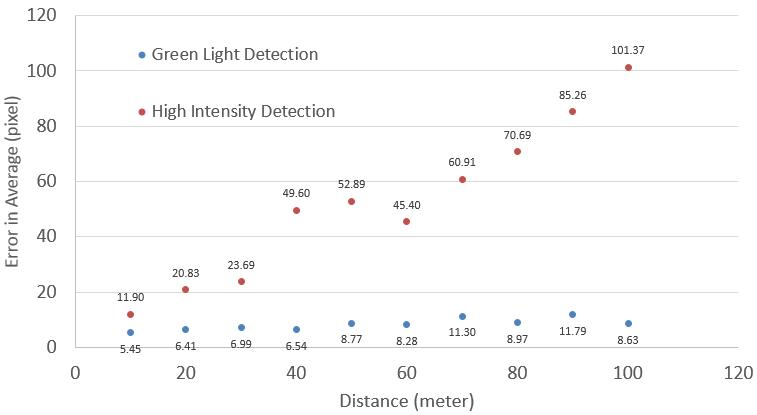
\includegraphics[scale = 0.6]{pics/dataday.jpg}
\end{center}
\end{table}

Direct sun light is too strong compared to the laser pointer, so it must be prevented. The illuminance of surrounding light in shadow is about $760,000LUX$, which is good enough for the green light detection to work. Table 6.1 shows the experiment results under daylight shadows. The high light intensity detection was defective beyond $30m$ while the green light detection worked properly all the time.  


\begin{table}[ht!]
\begin{center}
\caption{The Average Error at Night ($20LUX$)}
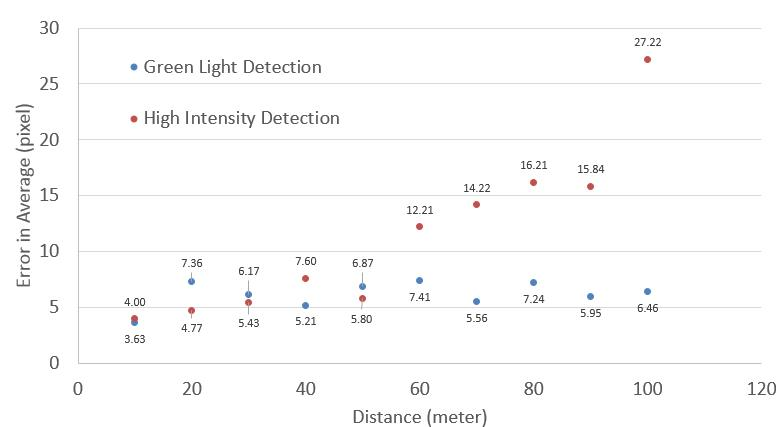
\includegraphics[scale = 0.6]{pics/datanight.jpg}
\end{center}
\end{table}

Table 6.2 shows the results at night for the same procedure of the experiment. The illuminace of surrounding light is only $20LUX$. Green light detection still worked all the time, but the high light intensity was slightly off beyond $50m$.

In both experiments, the green light detection was slightly unstable, especially during the night, because of the laser pointer. This common $5mW$ laser pointer scatters seriously as the range goes far. This starts to affect the detection from $70m$ and farther in the day, and detection is even more affected at night because under a weak surrounding light, any green light noise on the curtain will be detected. Therefore, a more precise laser pointer with less scattering at greater distances is necessary for the real device.
%激光在远距离散射严重

\section{Stepper Motor Control}

%\subsection{Motor Speed vs. Control Signal Frequency}

%\subsection{Motor speed vs. Input Current}

\subsection{Motor Speed}

The motor speed was measured with motor control code only, so that the image processing part will not slow the motor down. The motion of the motor was controlled directly by user input, and it ran at full speed. The time was counted in the program and the displacement was measured by a ruler. The loop ran for 500 cycles, and the time consumed was $3182114\mu s$, or about $3.13s$. The displacement measured was about $20cm$. The result is $6.39cm/s$.  

\subsection{Loop Speed}

Usually loop speed is insignificant, but it is considerable for a 900MHz CUP. The loop speed was measured in the program, so it is considered accurate. The motor control loop has a good run speed, which is $6260\mu s/loop$, but the image processing loop is much slower. Its loop speed is $170608\mu s/loop$, which means it takes about $0.17s$ for each loop. If both the image processing and motor control code run together, it will take $176868\mu s$ for each loop. It would need $44.217s$ to make a $10cm$ movement, which is unacceptable. Therefore, multi-thread programming is necessary. If the image processing and motor control parts run in two threads, the motor is able to run at full speed while the image processing part sends a command every $0.17s$. It would only need $1.56s$ to make a $10cm$ movement, which is much better.

%\subsection{Multi-thread Programming}

\subsection{Reaction Time}

The typical operating speed of a farm tractor is between 5 and 10$km/h$, which is about $1.39-2.78m/s$. The laser guidance system has to find and correct the error in a limited time. Since the loop speed for image processing is $0.17s/loop$, the queuing time for an incoming frame is from $0s$ to $0.17s$, and the analyzing time is $0.17s$. Hence the reaction time is $0.17-0.34s + 0.16cm/s$. For example, the time needed to correct a $5cm$ is $0.97-1.14s$. However, the tractor can move over $1m$ in this time window. Therefore, hardware more powerful than this prototype will be needed in the real device.


%\subsection{Vehicle Moving Speed Estimation}

%\section{Practical Application Parameters Prediction}
%预测实际情况中所需电子元件的参数
%通过 农机工作时的移动速度 和 实际需要的reaction time 
%推算出 马达扭矩,速度 以及 microprocessor的处理速度
%再通过 马达和microprocessor的功率 推算出所需电源
%预测 sliding track需要的长度
%预测 投影布的大小

\chapter{FUTURE IMPROVEMENT}

The buffer was designed as a linear buffer that can only provide the offset in the direction that is perpendicular to the direction in which the tractor is moving. However, the tractor cannot move left or right, it can only turn left or right. Therefore, after the sliding occurs, the tractor has to turn to make the correction. In other words, there are some small angles between the planned direction and the actual direction while tractor is moving. In order to cancel these angles, this design needs some improvements.

\section{Improvement to the Buffer}
\begin{figure}[ht!]
\begin{center}
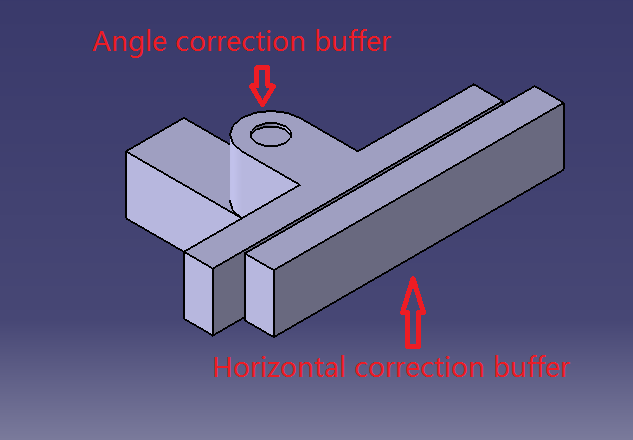
\includegraphics[scale = 0.8]{pics/improvedbuffer.png}
\caption{Improved Buffer}
\end{center}
\end{figure}
Based on the previous design, one more stepper motor needs to be installed, as Figure 7.1 shows, to provide the offset for the angle. The purpose of the stepper motor is to provide a vertical spin to correct the angle error while that tractor is turning. 

\section{Improvement to the Curtain}
\begin{figure}[ht!]
\begin{center}
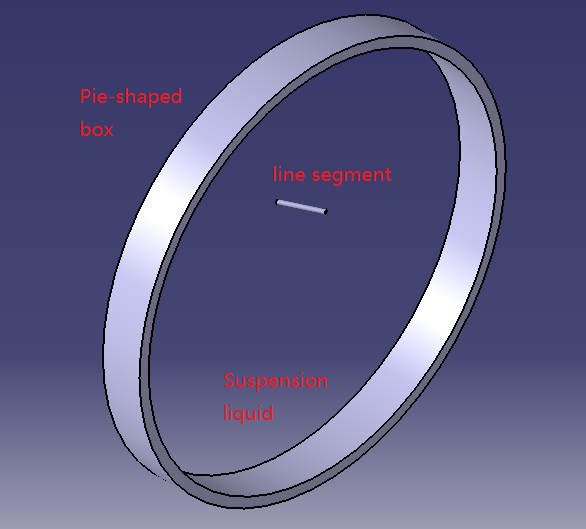
\includegraphics[scale = 0.8]{pics/improvedcurtain.png}
\caption{Improved Curtain}
\end{center}
\end{figure}
Previously, it was introduced that the curtain works like a projection screen. The only trace that the laser left is a spot. Under this situation, it is impossible to find the error angle just from one single spot. The new design for the curtain is a pie-shaped transparent plastic box filled with suspension liquid. Under the semi-transparent environment, the trace of the laser is no longer a spot, but a segment. (Figure 3.8) A segment provides more information than a single spot, and it is easier to find the angle with the direction and length of the segment.

\section{Improvement to the Algorithm}
Base on the developed color detection algorithm, the image captured by the camera shows a line segment. (Figure 3.9)
\begin{figure}[ht!]
\begin{center}
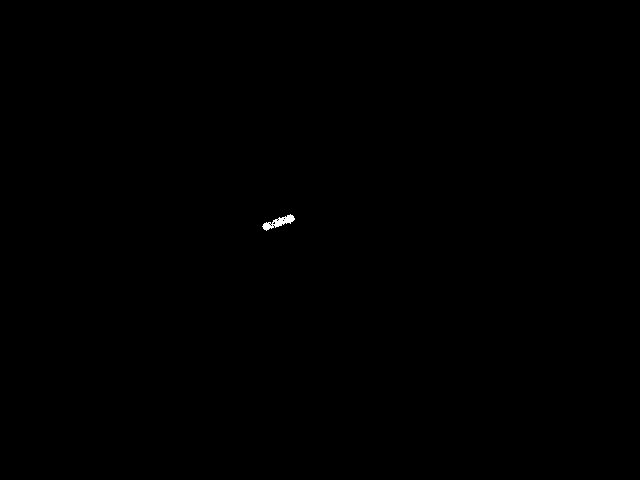
\includegraphics[scale = 0.6]{pics/segment.png}
\caption{Line Segment}
\end{center}
\end{figure}
The improved algorithm finds the angle by the following process. 
\subsection{Coordinates for Each End}

The camera is monitoring the curtain slightly upward, so according to the perspective rule, the upper right end of the segment is the front. For example, the coordinate of upper right end is $(292,217)$, and the coordinate for the lower left end is $(265, 227)$ in Figure 3.9.

\subsection{Projection Length of Segment}

With the coordinates of these two end points, the projection length can be calculated as below, and the unit is pixel. 
\begin{equation}
L = \sqrt{(292-265)^2+(217-227)^2} = 29 \quad pixels
\end{equation}

\subsection{Thickness of the Curtain}

Since the position and the size of the curtain are both fixed, thickness is a constant in this algorithm. This constant was found by taking a picture with the same distance and measuring the pixels on the picture. The thickness of the curtain is 56 $pixels$.

\subsection{Error Angle}

Since the projection length of the segment and the thickness of the curtain are known from the above calculations, the error angle can be calculated with trigonometric function according to the following:
\begin{equation}
Error Angle = tan^{-1}(\frac{29}{56}) = 27.38^o
\end{equation}

According to the perspective rule, the buffer was turned to the right 14.84 degrees. Therefore, this error angle can be corrected by turning the second stepper motor to the left 14.84 degrees. 

% Put chapter \include commands here.

\chapter{CONCLUSION}

\section{Introduction}
This paper introduced a new guidance system design for agricultural machinery. This design contains a buffer and a laser pointer. The buffer is a device that needs to be installed on a tractor attachment, and the laser pointer needs to be placed at the end of crop field rows facing to the back of the tractor. First, in order to use this guidance system, the laser must be put in the right position and face the right direction. Then the laser must be projected onto the curtain of the buffer. After the buffer has initialized, the tractor is ready for operation. This system is not only suitable for existing GPS-guided agricultural machinery, but it also works on machinery without any guidance systems on board in order to enhance the accuracy from $\pm$ 10 cm to $\pm$ 2 cm. The only difference is addition LEDs needs to be installed on the dashboard of the tractor. If the driver can drive at a low speed and handle the steering wheel carefully based on the signal on the dashboard, which is given by the laser guidance system, it is expected to have the same $\pm$ 2 cm accuracy. 

%使用这个设备能达到那些效果。为农业育种提供方便,为未来的无人农业提供先决条件。

\section{Technical Highlights}

\subsection{Local Laser Reference}
The guidance system introduced in this paper uses a laser as a local reference. A local reference is able to provide a more reliable guide because there are less noise factors. For instance, GPS is based on the distance measurement between several satellites and a receiver, and the high atmosphere has a significant affect on its accuracy. 

\subsection{Buffer}
The method that how this laser guidance system corrects error is to install a buffer to the tractor attachment. The method that current technology use to make corrections is to turn the steeling wheel of the tractor. This method is inefficient, because no matter how fast the correction can be made, there are deviations in the trajectory. However, deviations will never take place with the buffer installed on the tractor attachment. The buffer always stays at a relatively steady position with the laser reference. It allows the tractor to deviate for a little bit while keeping the trajectory on the right track before the tractor makes its correction.

\subsection{Image Processing}
The algorithm contains two parts. High-intensity detection is used when the tractor is close to the laser pointer. The laser pointer is designed to have range that is over 200 $m$, so it is very bright at a close distance. High-intensity detection provides a more stable detection because it is too bright to detect color. Once the color detection shows a stable result, high-intensity detection will be disabled. 

%利用摄像头来引导是趋势,摄像头成本低,易于改进,人就是靠视觉获取信息,同样机器也可以

\section{Feasibility}
The laser guidance system introduced in this paper is an add-on device to the current tractor attachments. Users does not need to buy new tractors or attachments, just the two parts of this device. Therefore, the cost is very low. However, the set-up procedure is a little bit complex. Therefore, it may not be the best choice to spread out to every farm because of the 76.2 $cm$ row spacing that is still mostly in use. The best place to apply this design is the experimental crop field, with the goal of finding the high performance breed. The seeding position is very strict, so that different breeds are comparable because of the identical growth environment of every plant. 

In the future, the row spacings will be as narrow as possible so that more crops can be planted, so high accuracy agriculture machinery is necessary for every corner of the world. The advantage of laser guidance systems is that every machinery on duty is able to upgrade. It is not necessary to buy a brand-new tractor that has a GPS guidance system on board and then upgrade based on the GPS. Therefore, laser guide system is a great choice for most of the developing country where GPS tractors are not popular. This is a very economical way for them to achieve the precision agriculture.


\section{Constraints}
The guidance system introduced in this paper is based on an image processing algorithm. Therefore, any condition that affects the camera will affect this system. The most common problem is dust caused by the running tractor. Heavy dust may block the laser light and cause the guidance system to lose reference. As for the laser light, a 5 $mW$ green laser pointer is in use for now and a higher power laser pointer may be used in the future to provide a farther distance reference. Therefore, safety is a big problem because the high-power laser can damage retinas at a close distance. Furthermore, it is very important to set up the laser pointer in the correct direction. A small error of angle will cause a big difference because of the long column distance. Based on these two reasons, it is necessary to have a trained operator. Last, because of limited resources and time, this guidance system is only designed for flat land. It will not work on sloping fields.


\section{Application for Other Areas}
Essentially, the design put forth by this paper is guidance system. Therefore, the laser guidance system can apply not only in agriculture machinery, but also in any other outdoor vehicles that need a precision guidance. In the aspect of agriculture, the buffer only stabilizes in a horizontal direction. In fact, the buffer can also stabilize in a vertical direction. This feature can be applied to a cart that moves fragile materials on a bumpy ground. For example, the outdoor AGVs with the laser guidance system are able to move fragile materials, such as glass, around the construction area just like indoor ones working in a factory. 


\section{Importance of Outdoor AGVs}
Outdoor AGVs was an essential and practical technology for the future of modern agriculture. Most of the current AGV are only is for indoor use, which is not applicable for outdoor environments. In outdoor conditions, various problems occur such as rough ground, unpredictable weather, and high expense of equipment, which is very different from indoor conditions. Furthermore, since most indoor AGV guidance systems require pre-set wires, magnets, or paints, it is very expensive and inconvenient to use them outdoors. Therefore, it is urgent to developed a feasible AGV for outdoor to use this paper mainly focuses on straight field rows. The significance of planting crops in a straight line is to produce the same condition for all areas in the experiment as well as to lay the foundation for further agriculture purposes; for example, straight rows reduce the work of irrigation by controlling the position of irrigation and creating convenience for agriculture robots. Hence, the development of laser guidance systems for AGVs can solve both problems mentioned and inspire more ideas for outdoor AGV researches.
%本文重点讨论了关于户外AGV在农业方面的应用,现在工厂有流水线,但是室外的农业却没有这么高效率。目前来说,传统的GPS农机或许在播种上能满足现在的需求。但是要满足育种试验田的播种需求,还是需要户外AGV。放眼未来,要实现想工厂流水线一样高效的无人农业,精准的播种是第一步也是非常重要的一步。

\section{Overview of Significance}
The laser guidance system introduced in this paper is an accurate and economic method to guide the outdoor vehicles. There are two devices in this guidance system; one of them is the laser pointer, and the other one is the buffer. The laser pointer emits a straight laser light that provides the reference for the guidance system. Its position is fixed on the ground and pointing to the direction that the vehicle needs to move. The buffer is installed on the vehicle to provide the guide. There is a camera on the buffer that is used to receive the laser light reference, and then the on board microprocessor analyzes the information by running the designed algorithm. Finally, the microprocessor sends action commands out. In this paper, these commands are sent to the buffer to stabilize the tractor attachment, as well as to the driver if there is no GPS guidance system on board. For other aspects, these commands not only guide the movement of the vehicle, but also can stabilize the cargo that was carried by the AGV. It is very useful if the AGV is transporting fragile materials on a dumpy ground.


\section{Limitations}
Laser light travels in a straight line, so this guidance system is only good at moving in a straight line. In order to make turns, it is better to have an additional guidance system on board, such as a GPS, to cooperate. Moreover, one laser pointer must to be set for each segment of the straight route. On the other hand, the laser guidance system will also be lost if the route is not monotonically up or down. Imagine a situation where a vehicle goes uphill and then downhill; the laser pointer can only guide the former movement. Therefore, there is a limitation in the geography of the working area.

The camera on the vehicle observes the laser light as a reference, but it might be hard to "see" the laser light under some situations. The observation will be affected by the surrounding lights. When this guidance system is used outdoors, the main factor that affects the laser light detection is strong sunlight. If the light intensity in the surroundings is too high, the laser light could be polluted so that green color cannot be detected. Therefore, it might be required to operate early in the morning or late in the afternoon, when the sun light is weak. 

\section{Further Improvement}
Based on the limitations, the laser guidance system can be improved in two ways in the future. First, the system could be adapted to diverse geographic working area. On the one hand, since some of crop fields are circular for the convenience of the giant irrigation sprinklers, it is better to plant the crops in the same shape. On the other hand, not all of the crop fields are flat. In fact, some farm land is in mountainous areas. It is necessary to make the guidance system able to work on every kind of farm. Second, the system could be adapted to reduce the affect from the strong sun light. Farming operations generally take place during the day. Furthermore, most of the crops require a very limited time window to be planted. In order to apply the laser guidance system widely, it would be more convenient if the guidance system were able to work properly at any time. 

%%
%  recommendations.tex  2007-02-06  Mark Senn  http://www.ecn.purdue.edu/~mark
%

\chapter{Recommendations}

Buy low.  Sell high.

%
%  bibliography.tex     June 3, 2002     Mark Senn
%
%  This is the bibliography for a simple, example thesis.
%

\bibliography{all}

% Use "\appendix" for one appendix or "\appendices" for more than one
%\appendix
%\begin{algorithm}
\caption{Motor Control}
\begin{algorithmic} 
\IF {$point.x \leq 310$}
\STATE {$rotate(clockwise)$}
\ELSIF {$point.x \geq 330$}
\STATE {$rotate(counterclockwise)$}
\ELSE
\STATE {do nothing}
\ENDIF 
%\STATE
\STATE {Function $rotate$($direction$)}
\STATE {$pins = 0, 1, 2, 3$}
\STATE {$sequence[8] = 1, 1, 0, 0 \Rightarrow 0, 1, 0, 0 \Rightarrow 0, 1, 1, 0 \Rightarrow 0, 0, 1, 0 \Rightarrow 0, 0, 1, 1 \Rightarrow 0, 0, 0, 1 \Rightarrow 1, 0, 0, 1 \Rightarrow  1, 0, 0, 0$}
%\STATE {$$}
%\STATE {$\quad $}
%\STATE {$\qquad \qquad \quad \quad \quad 0, 1, 1, 0$}
%\STATE {$0, 0, 1, 0$}
%\STATE {$0, 0, 1, 1$}
%\STATE {$0, 0, 0, 1$}
%\STATE {$1, 0, 0, 1$}
%\STATE {$1, 0, 0, 0$} 
\IF {$direction = clockwise$}
\FOR {$i = 1 \rightarrow 8$}
\STATE {$pins = sequence[i]$}
\ENDFOR
\ENDIF
\IF {$direction = counterclockwise$}
\FOR {$i = 8 \rightarrow 1$}
\STATE {$pins = sequence[i]$}
\ENDFOR
\ENDIF
\end{algorithmic}
\end{algorithm}
%\appendices


% A vita is optional for masters theses
% and required for doctoral dissertations.

%%
%  vita.tex   2003.07.23  14:59:33   Mark Senn <mds@purdue.edu>
%
%  This is the vita for a simple, example thesis.
%
%  A vita is required only in a doctoral dissertation.
%

\begin{vita}
    [Put a brief autobiographical sketch here.]
\end{vita}

\end{document}
